\documentclass[11pt]{report}



\usepackage[margin=1.1in]{geometry}

%\usepackage{fontspec}
%\setmainfont{Arial}
\usepackage{setspace}

\usepackage{cite}
\usepackage{adjustbox}
\usepackage[font={small}, labelfont = {bf}]{caption}
\usepackage{graphicx}
\usepackage{array}
\usepackage{subcaption}
\usepackage{amsmath}
\usepackage{amssymb}
\usepackage{setspace}
\usepackage{gensymb}
\usepackage{tablefootnote}
\usepackage[T1]{fontenc}
\usepackage{helvet}
\usepackage[utf8]{inputenc}
\usepackage{subcaption}
\usepackage{float} 
\usepackage{subfloat} 
\usepackage{longtable}
\usepackage{multirow}
\usepackage{booktabs}
\usepackage[justification=centering]{caption}
\usepackage{pdfpages}

\renewcommand{\familydefault}{\sfdefault}

%\renewcommand{\bibname}{References}
\newcolumntype{?}{!{\vrule width 1pt}}

\makeatletter
\newcommand{\thickhline}{%
    \noalign {\ifnum 0=`}\fi \hrule height 1pt
    \futurelet \reserved@a \@xhline
}
\newcolumntype{"}{@{\hskip\tabcolsep\vrule width 1pt\hskip\tabcolsep}}
\makeatother


\newcounter{FootnoteCounter} 
\stepcounter{FootnoteCounter} % Add one to counter (initialised at zero)
%\footnotemark[\arabic{FootnoteCounter}] // Place the footnote number in the text
%\footnotetext[\arabic{FootnoteCounter}]{Example footnote} // Set the text to be displayed with this instance of footnote
%\stepcounter{FootnoteCounter} // Increment the counter for the next useage.

\usepackage{fancyhdr}
 
\usepackage{pdfpages}
 
 
\pagestyle{fancy}

\fancyfoot[C]{\sffamily\fontsize{9pt}{9pt}\selectfont\thepage}

\setlength{\textfloatsep}{\baselineskip + 0.2\baselineskip - 0.1\baselineskip}

\numberwithin{equation}{chapter}
\doublespace


\begin{document}

\begin{titlepage}

\newcommand{\HRule}{\rule{\linewidth}{0.5mm}} % Defines a new command for the horizontal lines, change thickness here

\center % Center everything on the page
 

%----------------------------------------------------------------------------------------
%	TITLE SECTION
%----------------------------------------------------------------------------------------

\HRule \\[0.4cm]
{ \huge \bfseries The Future of Work -- \\ Machine Learning and Employment}\\[0.4cm] % Title of your document
\HRule \\[1.5cm]

%----------------------------------------------------------------------------------------
%	HEADING SECTIONS
%----------------------------------------------------------------------------------------

%\textsc{\LARGE University of Oxford}\\[1.5cm] % Name of your university/college

\includegraphics[scale = 0.2]{logo.jpg}\\[1cm] % Include a department/university logo - this will require the graphicx package
 
%\textsc{\Large St-Hugh's College}\\[0.5cm] % Major heading such as course name
 
%----------------------------------------------------------------------------------------
%	AUTHOR SECTION
%----------------------------------------------------------------------------------------


% If you don't want a supervisor, uncomment the two lines below and remove the section above
\Large \textbf{Mu Chen}\\ % Your name
\Large St Hugh's College\\[3cm]

\Large Supervisor: Michael Osborne\\
\Large Department of Engineering Science\\
\Large University of Oxford\\[1cm]

%----------------------------------------------------------------------------------------
%	DATE SECTION
%----------------------------------------------------------------------------------------

{\large Trinity Term 2016}\\[3cm] % Date, change the \today to a set date if you want to be precise


%----------------------------------------------------------------------------------------

\vfill % Fill the rest of the page with whitespace

\end{titlepage}
\newpage

\includepdf[pages=-]{Declaration.pdf}

\pagenumbering{roman}
\newpage
%\maketitle
\section*{Abstract}
The goal of the project is to build upon the work of \cite{frey2013future} about the future of employment and further investigates how susceptibilities of jobs has affected employment since 1980s.  Machine learning techniques are applied to two sets of data, each containing a list of job descriptors from 1977 and 2010 respectively, to estimate the probability of computerisation for every occupation in each time period. These estimations are then examined on labor force market changes. The result proves the conclusion of many others work\cite{david2001skill}\cite{levy2012new}, from a probability point of view, that computer capital is substitutable for workers involving routine tasks -- tasks following programmable rules, but not a threaten to workers in non-routine jobs in general, although there are indications that some non-routine jobs such as non-routine manual jobs are no longer safe.

\newpage
\section*{Acknowledgement}
First I would like to thank my supervisor, Michael Osborne, for his generous support throughout this project. His invaluable advices and his brilliant lectures have all helped me understand the subject and finish the project. I would also like to thank Carl Frey from Oxford Martin School for his essential information on employment data that forms the core of my experiment data. Finally, I would like to acknowledge the reference of GP regression code written by Mark Ebden, where I started developing my own GP program. 

\newpage 
\rhead{Table of Contents}
\lhead{} 
 
\tableofcontents

\begin{spacing}{2}

\newpage
\pagenumbering{arabic}
\setcounter{page}{1}



\chapter{Introduction}
\rhead{Introduction}
The question of how technology could influence employment has been a popular issue for quite a long time\cite{machin1998}. Since 1990s, it was believed that technological changes have favoured the more skilled workers while reduced the demand for less skilled workers\cite{bound1989changes}. Nowadays, with much faster development of technologies especially in automation technology, it is very likely for people to believe that less human worker is required. If it is true, could it be the major cause for lower employment rate? Will the development of technology make more people jobless? Or is it just a temporary phenomenon? 

Many works have been done to reveal the impact of technology on labor force. Brynjolfsson and McAfee\cite{brynjolfsson2012race} believed that technology has contributed to persistent high employment rate. They observed that, after the Great Recession\footnote{A period of economic decline observed in world markets during the late 2000s}, when companies are expected to take in more workers, they bought more computers. The only reason behind is that computer capital became cheaper than human worker. 

Although it is commonly believed that there are jobs in which humans are not replaceable\cite{levy2012new}, there are large amount of jobs that have already been automated. Past works have proven that computers are substitutive for jobs mainly involving routine tasks\cite{david2001skill}. However, with recent development in artificial intelligence such as pattern recognition, some non-routine tasks, especially non-routine manual tasks are no longer invincible.  It is not impossible that other non-routine tasks would be manageable by computers in the future.

In this project, a GP is run on two sets of data, one includes variables related to 2010 occupations, the other includes tasks performed for each occupation in 1977\cite{david2001skill}. The training set of 2010 occupations are hand-labeled data from \cite{frey2013future}. The same labels are transferred to 1990 occupations through official crosswalk files from IPUMS\cite{SOC2010_2000},\cite{SOC2000_OCC}\cite{OCC2000_1990}. These two sets of data are run with GP classification MATLAB program separately. The results are then compared with each other as well as with historical labor force data\cite{IPUMS1990}. 

The following chapters will present the details of how machine learning is used for studying the relation between technology development and employment. Chapter  \ref{GP} will introduce the basics of the Gaussian process and the implementation details of Gaussian process classification. Then Chapter \ref{GP_for_employment} will be talking about how employment data sets from 2010 and 1980  are used in GP and what conclusions could we make from the results. Finally Appendix \ref{App:results_all} includes some numerical results of the project.




\newpage
\chapter{Gaussian Process}
\label{GP}
\rhead{Gaussian Process}
Gaussian Process(GP) is a modelling method in which all variables are assumed to follow normal distribution. Any finite combination of input spaces also has a joint Gaussian distribution. Thus the distribution of a Gaussian Process model can be seen as the infinite-dimensional generalization of the multivariate normal distribution. 

A Gaussian Process has several advantages over other models. First, its non-parametric modelling process gives it flexibility. It is not restricted by the expressivity of a set of parameters of fixed size. Second, a Gaussian Process is particularly useful for small data sets because the priors in this family can give characteristics you want (such as smoothness and periodicity), at the same time keeping a fine fit to the data.  

By definition, a Gaussian Process $f(x)$ is specified by a mean function and a covariance function, denoted as  

\[f(x) \sim GP(\mu(x),K(x,x))\]

where

\begin{align}
\mu(x) &= \mathbb{E}(f(x))\\
k(x,x\prime) &= \mathbb{E}((f(x) - \mu(x)(f(x\prime) - \mu(x\prime)) 
\end{align}

Both the mean and covariance function are the choice of user and can have crucial effects on the final Gaussian process distribution.

To describe how all the input points are related together we use the covariance matrix defined as 

\begin{equation}
K(x,x\prime) = \left[\begin{array}{cccc}
k(x_1,x_1) & k(x_1,x_2) & \cdots & k(x_1,x_n)\\
k(x_2,x_1) & k(x_2,x_2) & \cdots & k(x_2,x_n)\\
\vdots & \vdots & \ddots & \vdots\\
K(x_n,x_1) & k(x_n,x_2) & \cdots & k(x_n,x_n)\\

\end{array}\right].
\end{equation}

\subsubsection{Mean Function}
The prior mean function $\mu(x)$ describes the beliefs in output y(x) before any observations are made. The most popular choices of $\mu$ includes 0 and other constants. More complicated mean functions can be defined by using certain parameters based on domain knowledge. However, one should always be careful in selecting the mean function since it is what specifies extrapolation behaviour.   

\subsubsection{Covariance Function}
Many characteristics such as smoothness, stationarity, and periodicity can be integrated in covariance function. It describes how individual observations are related to each other. In reverse, learning in Gaussian Process also defines the properties of covariance function, giving us the model that can be used for upcoming predictions.   

One common choice is the squared exponential covariance function
\[k(x,x\prime) = \sigma_f^2\operatorname{exp}\left[-\frac{(x-x\prime)^2}{2l^2}\right]\]
where $l$ is the lengthscale representing how far a certain training point could affect the predictions. It is suitable for smooth data. One thing to notice is that the $k(x,x\prime)$ is actually the covariance between $y$ and $y\prime$, corresponding to the output of $x$ and $x\prime$ respectively. Other covariance functions such as rational quadratic function can be useful for data that is smooth over a range of length scales.

The Matérn class of covariance functions is another important branch of covariance functions. They take the form of 
\[K_{Matérn}(x,x\prime) = \lambda^2 \frac{2^{1-\nu}}{\Gamma(\nu)}\left(\frac{\sqrt{2\nu} d(x,x\prime)}{l}\right)^\nu K_\nu \left(\frac{\sqrt{2\nu} d(x,x\prime)}{l}\right)\]
where $d(x,x\prime)$ is the distance between $x$ and $x\prime$. This type of covariance is normally used for functions of varying smoothness. 

Periodicity can be added by using the periodic covariance of the form
\[K_P(x,x\prime) = \lambda^2 \operatorname{exp}\left(- \frac{2sin^2\left(\pi d(x,x\prime)/\rho\right)}{\omega}\right)\] 
where $\rho$ determines the period and $\omega$ gives the roughness.

Covariance functions can be combined to give multi-character correlations. For example, if we know that it requires both periodicity and smoothness in the distribution, the multiplication of squared exponential function and periodic function can be used. If the prior information is that either periodicity or smoothness exists, the addition of the above two functions suits better. Similar techniques can be applied to distributions that are known to be the sum of independent functions or the product of independent functions.

One thing to notice is that most of the covariance functions involves computing the distance between input points. This distance could either simply be the euclidean distance $d_E(x,x\prime) = \sqrt{\sum\limits_{i=1}^n(x_i - x_i\prime)^2}$ or the weighted distance defined by $d_w(x,x\prime) = \sqrt{\sum\limits_{i=1}^n\frac{(x_i - x_i\prime)^2}{w_i^2}}$.


\section{Gaussian Process Regression}
\rhead{Regression}

GP Regression by its name is the process of finding a model to fit a data set using a Gaussian Process. In practice, it is often the case that the output data we collected are noise corrupted. eg. $y = f(x)+ \epsilon$. If we assume the noise $\epsilon$ is Gaussian with variance $\sigma_n^2$ and independent in each observation, covariance between observations then becomes

\begin{equation}
\label{cov_y}
\operatorname{cov}(y,y\prime) = k(x,x\prime) + \sigma_n^2\delta
\end{equation}

where $\delta$ is the Kronecker delta function which becomes 1 when $x = x\prime$ and 0 otherwise.

\begin{figure}[h]
\centering
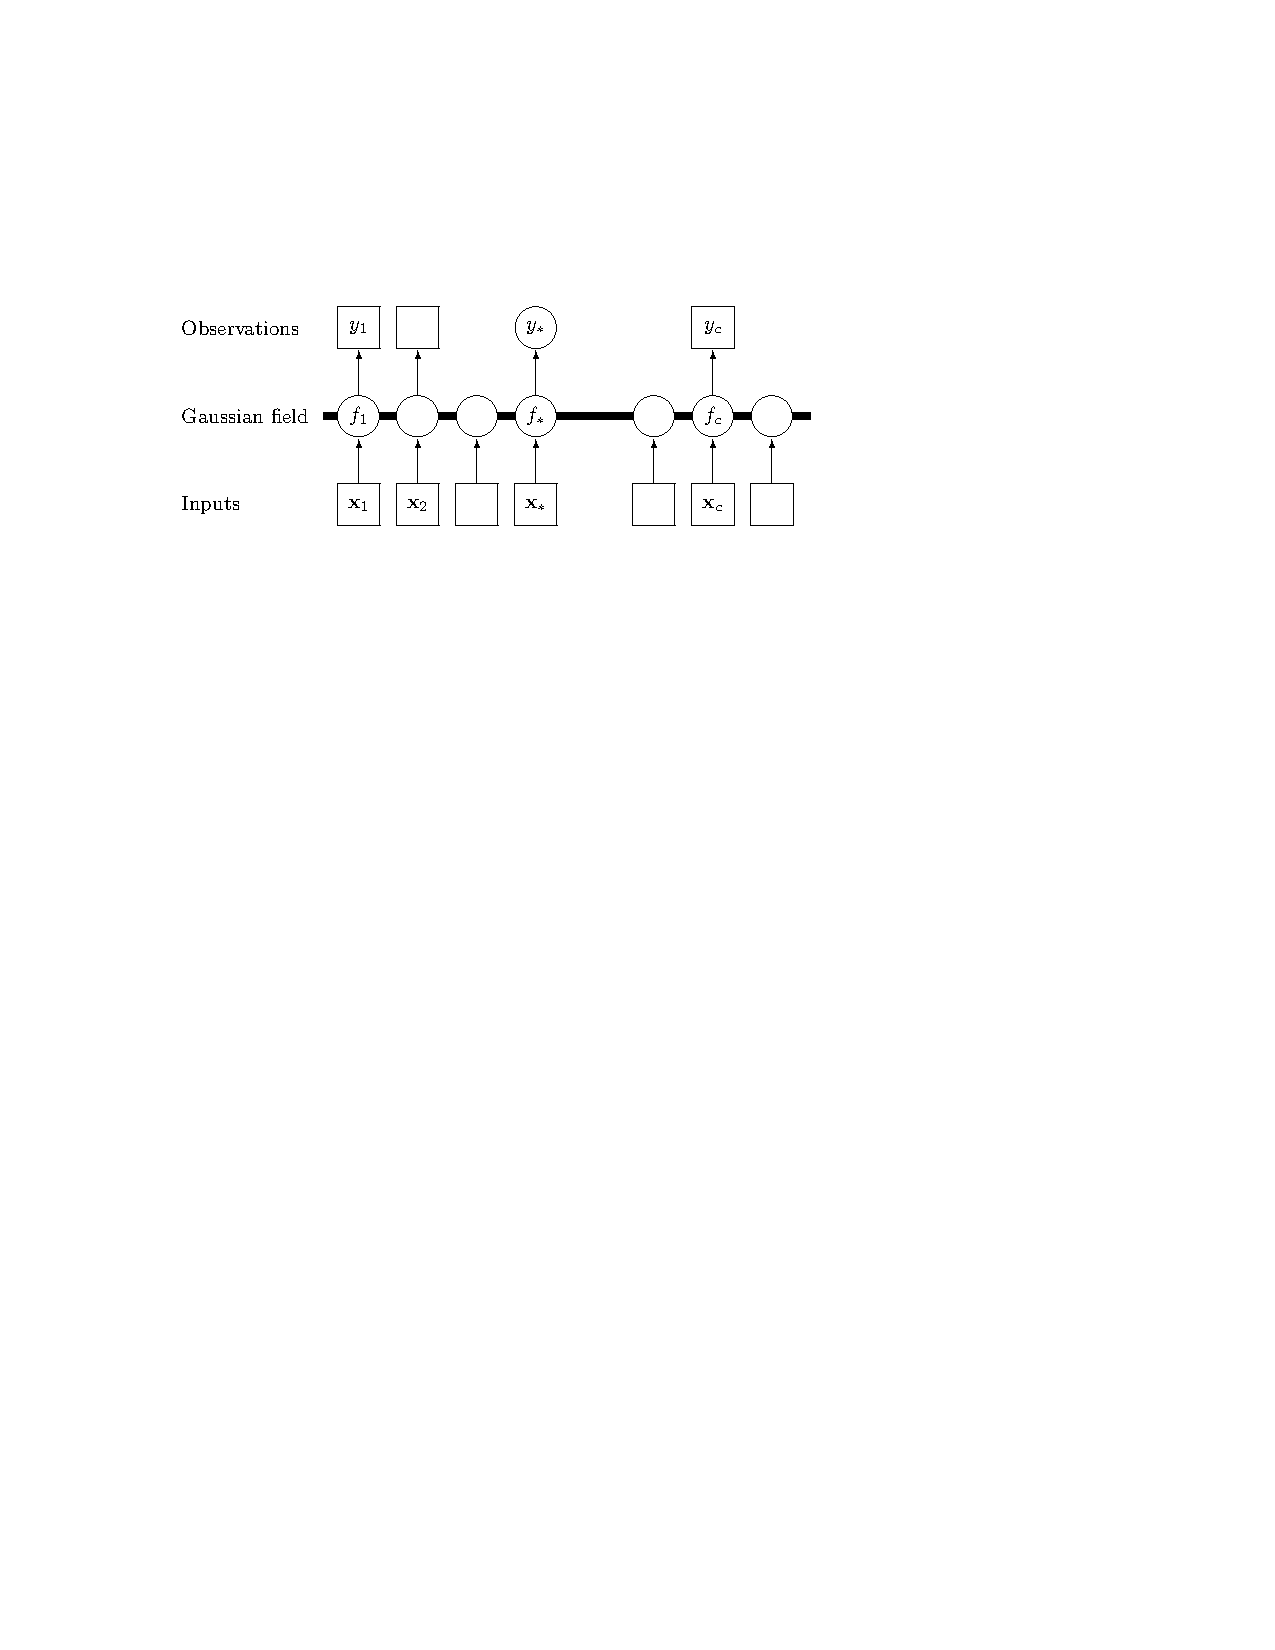
\includegraphics[scale=1.0]{Regression_model.pdf}
\label{regression_model}
\caption{The relation between input ($x$), observational output ($y$), and the latent variable ($f$). \newline Figure from \cite{RW}}
\end{figure}


\subsection{MLE and MAP for Setting Hyperparameters}
Although Gaussian Process is non-parametric, we still need to find the hyperparameters which define the mean and covariance functions. In fact, the objective of finding hyperparameters other than the parameters for model itself gives us more freedom in defining the distribution function. 

According to Bayes' rule,

\[\mbox{posterior} = \frac{\mbox{likelihood}\times \mbox{prior}}{\mbox{marginal likelihood}}\]

if $\theta$ is the collection of all hyperparameters

\[p(\theta|X,y) = \frac{p(y|X,\theta)p(\theta)}{p(y|X)}\]

where the marginal likelihood $p(y|X)$ is given by 

\begin{equation}
\label{pY_X}
p(y|X) = \int{p(y|X,\theta)p(\theta)}d\theta
\end{equation}

The MLE and MAP estimates the integrals by approximating the likelihood $p(y|X,\theta)$ and posterior $p(\theta|X,y)$ respectively as delta function of $\theta$. Indeed, the differences between the approximation and the real function value may have an negative impact on our final results. However, as the approximations are on hyperparameters, which only affects mean and covariance function but not the function parameters (function values), the negative impact arisen from MLE or MAP is reduced as they propagate to the actual function values.

Note that in equation (\ref{pY_X}), $\theta$ is marginalised out therefore $p(y|X)$ is independent of the values of theta. The maximum a posterior estimate of $\theta$ happens when $p(\theta|X,y)$ is maximised. Since $p(\theta|X,y)$ is proportional to $p(y|X,\theta)$, if we have little knowledge about the prior information of $\theta$, finding the maximum of the posterior is equivalent to obtaining the value of $\theta$ that maximises $p(y|X,\theta)$. $p(y|X,\theta)$ can be written as the integration of latent variable f

\begin{equation}
\label{theta_likelihood}
p(y|X,\theta) = \int{p(y|f,X,\theta)p(f|X,\theta)}df.
\end{equation}

In Gaussian Process model we assume that $p(f|X,\theta)$ is a Gaussian with mean 0 and variance $K$. A multi-variate Gaussian probability density function can be written as 

\[\mathcal{N}(\mathbf{x},\mathbf{\mu},\mathbf{\Sigma}) = \frac{1}{\sqrt{|2\pi\mathbf{\Sigma}|}}\operatorname{exp}\left(-\frac{1}{2}(\mathbf{x} - \mathbf{\mu})^T\mathbf{\Sigma}^{-1}(\mathbf{x} - \mathbf{\mu})\right)\]

therefore we have

\begin{equation}
\label{f_posterior}
\operatorname{log}p(f|X,\theta) = -\frac{1}{2}f^TK^{-1}f-\frac{1}{2}\operatorname{log}|K| - \frac{n}{2}\operatorname{log}2\pi
\end{equation}

also we know that $y|f\sim \mathcal{N}\left(f,\sigma_n^2 I\right)$, combining it with the above equation we get

\begin{equation}
\operatorname{log}p(y|X,\theta) = -\frac{1}{2}y^T(K+\sigma_n^2 I)^{-1}y - \frac{1}{2}\operatorname{log}\left|K+\sigma_n^2 I\right|- \frac{n}{2}\operatorname{log}2\pi
\end{equation}

This is the final objective function to be maximised. The covariance of $y$ from this equation is $K+\sigma_n^2$, which is also consistent with the covariance of $y$ we derived earlier in equation (\ref{cov_y}) where a noise term is added to the diagonal of $K$.


\subsection{Predictions}
After finding the optimised hyperparameters, predictions can be made by substituting the new inputs into the Gaussian Process model defined by mean and covariance function with the optimised parameters. The joint distribution of training data with no noise can be written as 

\begin{equation}
\left[\begin{array}{c} 
\mathbf{f} \\
\mathbf{f}_\ast \end{array}
 \right] \sim \mathcal{N} 
 \left(\mu(X), \left[\begin{array}{cc}
 K(X, X) & K(X, X_\ast)\\
 K(X_\ast, X) & K(X_\ast, X_\ast)
 \end{array}\right]\right)
\end{equation} 

Where $\mathbf{f}_\ast$ denotes the predictions in $f$ domain. Similarly, distribution of noisy training data can be expressed as

\begin{equation}
\left[\begin{array}{c} 
\mathbf{y}\\
\mathbf{f}_\ast \end{array}
 \right] \sim \mathcal{N} 
 \left(\mu(X), \left[\begin{array}{cc}
 K(X, X) + \sigma_n^2I & K(X, X_\ast)\\
 K(X_\ast, X) & K(X_\ast, X_\ast)
 \end{array}\right]\right)
\end{equation}

Then the distribution of $\mathbf{f}_\ast$ conditioned on $X, X_\ast$ and $\mathbf{f}$ follows a Gaussian with mean and variance as below

\begin{align}
\label{predictive_mean_noise_free}
\bar{\mathbf{f}}_\ast & = \mu(X_\ast) + K(X_\ast, X)K(X,X)^{-1}(\mathbf{f} - \mu(X))
\\
\label{predictive_covariance_noise_free}
\operatorname{cov}(\mathbf{f}_\ast) & = K(X_\ast, X_\ast) - K(X_\ast, X)K(X, X)^{-1}K(X, X_\ast)
\end{align}
 
and the noisy version,
\begin{align}
\bar{\mathbf{f}}_\ast & = \mu(X_\ast) + K(X_\ast, X)[K(X,X) + \sigma_n^2I]^{-1}(\mathbf{y} - \mu (X))
\\
\operatorname{cov}(\mathbf{f}_\ast) & = K(X_\ast, X_\ast) - K(X_\ast, X)[K(X,X) + \sigma_n^2I]^{-1}K(X, X_\ast)
\end{align}

\begin{figure}[h]
\centering
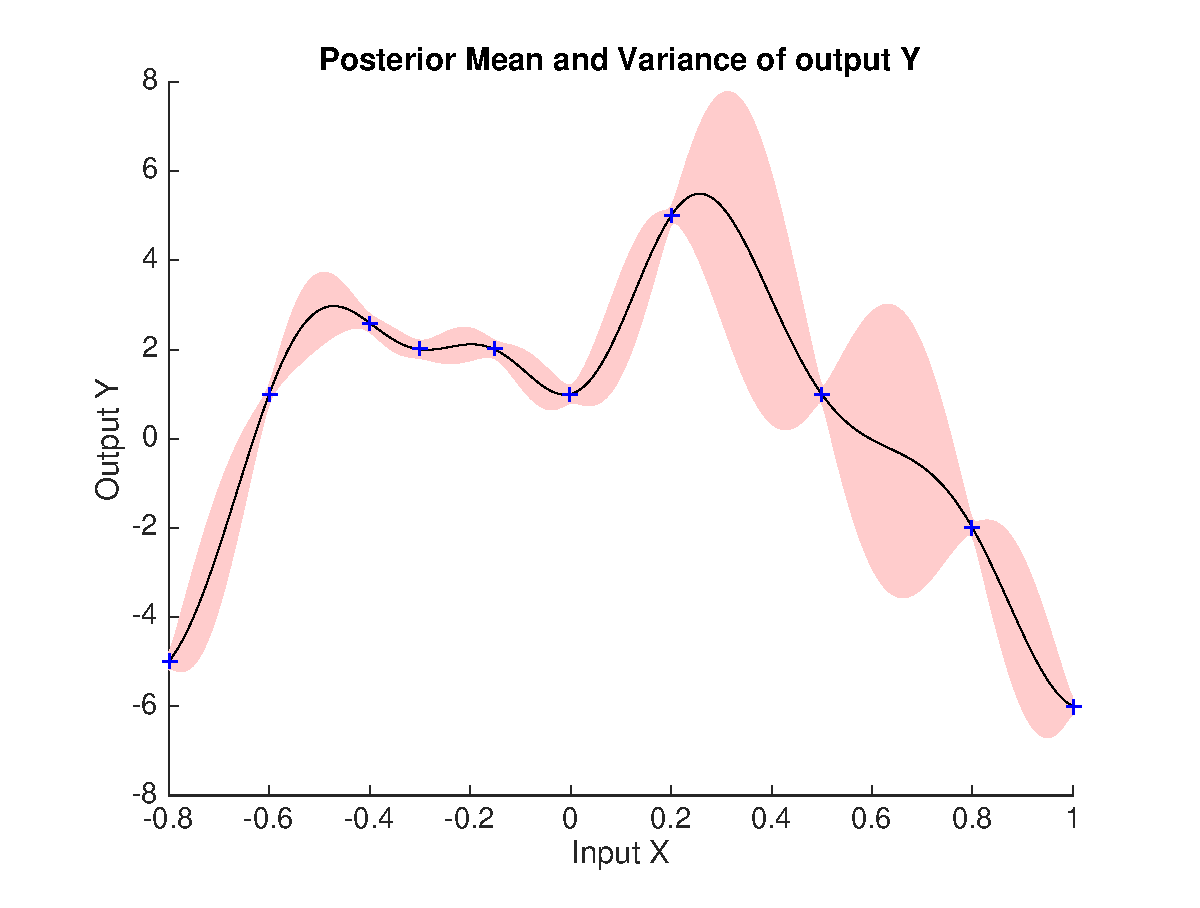
\includegraphics[scale = 0.55]{RegressionPlot1D.eps}
\label{regression_1D_plot}
\caption{Example plot of Regression with 1D input and output. Blue points represent the training set. Red region represents the variance of prediction. Note that the variance at the training points is almost reduced to zero as there is little uncertainty at these points (they are actually zero in noise free cases). The further way from training points, the more uncertain predictions become.}
\end{figure}

\subsection{Computational Issues}

\subsubsection{Conditioning on Covariance Matrix}
Covariance matrix $K$ has to be positive semi-definite for its consequential steps to be numerically stable. However, when the input data is so closed to each other compared to the length scale used, adjacent rows in $K$ might become the same under limited significant figures, making the matrix not full rank anymore.

This problem is avoided in regression problems by adding noise. While in classification problems that we are going to talk about later, artificial noise, also called jitters, has to be added. The amount of jitters needed differs by data, and user is required to adjust its size until $K$ becomes positive definite.

\subsubsection{Cholesky Decomposition}
For large data sets, a Gaussian Process can be very slow. The computation on large covariance matrix makes it highly time consuming. The most expensive computation is the inversion of $K$. Cholesky decomposition is one way to tackle this problem. It decomposes a positive definite matrix into the product of two triangular matrices

\begin{equation}
K = LL^T = U^TU
\end{equation}

where $L$ is a lower triangular matrix and $U$ is an upper triangular matrix. The inverse of $K$ can simply be computed by

\begin{equation}
K^{-1} = L^{-T}L^{-1} = U^{-1}U^{-T}.
\end{equation}

It is much faster to compute the inverse of a triangular matrix, giving a reduction in computation complexity from $\mathcal{O}(n^3)$ to $\mathcal{O}(\frac{1}{3}n^3)$\cite{marelli2015distributed}. In addition, matrix inversion based on cholesky decomposition is more numerically stable.  


\subsubsection{Partial Derivatives of Hyperparameters}
To optimise the hyperparameters using Newton's method, we need to compute the gradients of log likelihood of $\theta$ w.r.t. the hyperparameters $\theta_i$, given by 
 
\begin{equation}
\begin{split}
\frac{\partial}{\partial \theta_i} \operatorname{log}p(y|X,\theta) & = \frac{1}{2}y^T K^{-1}\frac{\partial K}{\partial \theta_i}K^{-1}y \, - \, \frac{1}{2}tr(K^{-1}\frac{\partial K}{\partial \theta_i}) \\ & = \frac{1}{2}tr\big( (\alpha\alpha^T - K^{-1})\frac{\partial K}{\partial \theta_i}\big) \quad\quad\quad \mbox{where}\quad\alpha = K^{-1}y
\end{split}
\end{equation}

One thing to notice is that many of the parameters, such as lengthscale and frequency, are always positive. Therefore it is more convenient to optimise over their logarithms other than themselves. e.g $\theta = \operatorname{log}\theta$. 









\section{Gaussian Process Classification}
\rhead{Classification}
Gaussian Process classification can be simply derived from GP regression except for the fact that outputs are discrete numbers representing class labels instead of continuous numbers in regression. Typically class labels are 1 and -1 for binary class problems. However, we do get a continuous intermediate function before the final label is decided. This is the latent variable on which regression is applied. Then the result of regression will be 'squashed' into range [0,1] to give the probability of a certain class.


\subsection{The Squashing Function}
\label{sigmoid function}
The squashing function can be any sigmoid function. Two typical sigmoid functions are logistic function $\lambda (f) = 1/(1 + \operatorname{exp}(-y_if_i))$ and cumulative Gaussian function $\Phi (f) $. Inference is hence divided into two steps. First is to compute  the distribution of the prediction latent variable $f_*$ in terms of previous observations 

\begin{equation}
\label{classification_prediction}
p(\boldsymbol f_*|\boldsymbol X,\boldsymbol y,\boldsymbol x_*) = \int p(\boldsymbol f_*|\boldsymbol X,\boldsymbol x_*,\boldsymbol f)p(\boldsymbol f|\boldsymbol X,\boldsymbol y)\ d\boldsymbol f
\end{equation}

where \(p(\boldsymbol f|\boldsymbol X,\boldsymbol y) = {p(\boldsymbol y|\boldsymbol f)p(\boldsymbol f|\boldsymbol X)}/{p(\boldsymbol y|\boldsymbol X)}\) is the posterior of latent variables $\boldsymbol f$, which is estimated by MAP with respect to hyperparameters($l$ and $\sigma_f$).

Then the probabilistic prediction is estimated by substitute the latent f into sigmoid function and average over 

\begin{equation}
\label{predictive_probability}
\bar{\pi}_* \triangleq p(y_* = +1|X,y,x_*) = \int \sigma (f_*)p(f_*|X,y,x_*) df_*
\end{equation}


\subsection{Laplace Approximation}

In the case of regression (equation \ref{theta_likelihood}), we assumed that both the likelihood $p(y|f)$ and the posterior over latent variable $p(f|X,\theta)$ are Gaussian. The integral for finding $p(y|X,\theta)$ and the prediction can be computed analytically. However, in classification, the non-Gaussian likelihood and the posterior of latent function make the integral (equation (\ref{classification_prediction})) not analytically tractable. Laplace's approximation can be used to approximate these two terms by doing a second order Taylor expansion of the logarithm around its maximum point. 

The Gaussian approximation of the posterior of $f$ can be obtained by:


\begin{equation}\label{LaplaceApp}
q(f|X,y) = \mathcal{N}(f|\hat{f},A^{-1}) \propto \operatorname{exp}(-\frac{1}{2}(f-\hat{f})^T A(f-\hat{f})) \,\sim\, p(f|X,y)
\end{equation}

where $\hat{f} = \operatorname{argmax_f} p(f|X,y)$ and $A = -\bigtriangledown\bigtriangledown \operatorname{log}p(f|X,y)|_{f=\hat{f}}$ is the Hessian of negative log posterior.


The reason we choose Laplace's approximation here is that it is more likely to give a better approximation than MLE or MAP\cite{azevedo1994laplace}. Although it may still be inappropriate for the true shape of the data: the peak can be much sharper or flatter than what the approximation described. 

%\begin{equation}\label{LaplaceApp_prediction}
%q(f_*|X,y, x_*) = \mathcal{N}(f|\hat{f},A^{-1}) \propto \operatorname{exp}(-\frac{1}{2}(f-\hat{f})^T A(f-\hat{f})) \,\sim\, p(f_*|X,y, x_*)
%\end{equation}


\section{Implementation}
\rhead{Implementation}
%%The project is mainly focused on classification problem, where the input is the measurements of each job and the output is the class label indicating whether the job would be automated or not.

\subsection{Optimising the latent variable}
By Bayes' rule
\[
p(\boldsymbol f|\boldsymbol X,\boldsymbol y) = {p(\boldsymbol y|\boldsymbol f)p(\boldsymbol f|\boldsymbol X)}/{p(\boldsymbol y|\boldsymbol X)} 
\]

We need to find the $\hat{f}$ that maximises $p(f|X,y)$. Also, $p(y|X)$ is independent of $f$, only the numerator need to be considered. Take the logarithm of $p(f|X,y)$ we get

\begin{equation}
\begin{split}
\Psi(f) & = \operatorname{log}p(f|X,y) \\
& = \operatorname{log}p(y|f) + \operatorname{log}p(f|X) \\
& = \operatorname{log}p(y|f) + \frac{1}{2}f^TK^{-1}f - \frac{1}{2}\operatorname{log}|K| - \frac{n}{2}\operatorname{log}2\pi
\end{split}
\end{equation}

and its derivatives w.r.t. $f$:

\begin{align}
\nabla\Psi(f) & = \nabla\operatorname{log}p(y|f) - K^{-1}f \\
\nabla\nabla\Psi(f) & = \nabla\nabla\operatorname{log}p(y|f) - K^{-1} = -W - K^{-1}
\end{align}

where $W$ is the second derivative of negative log likelihood of $f$. Since we know that $y_i$ depends on $f_i$ only, $W$ is a diagonal matrix. The best latent f can then be found at $\nabla\Psi = 0$, which gives 

\begin{equation}
\label{optimised_f}
\hat{f} = K(\nabla \operatorname{log}p(y|\hat{f}))
\end{equation}

This is a non-linear function therefore can be solved by Newton's method. Commonly used convergence criteria include the difference between successive values of $\Psi (f)$, the magnitude of gradient vector $\nabla\Psi (f)$ or the changes between values of $f$. In practice, the convergence of objective function is assured by checking that each iteration gives an increase in $\Psi (f)$. If not, a smaller step change in $f$ should be used. 

\begin{figure}
\centering
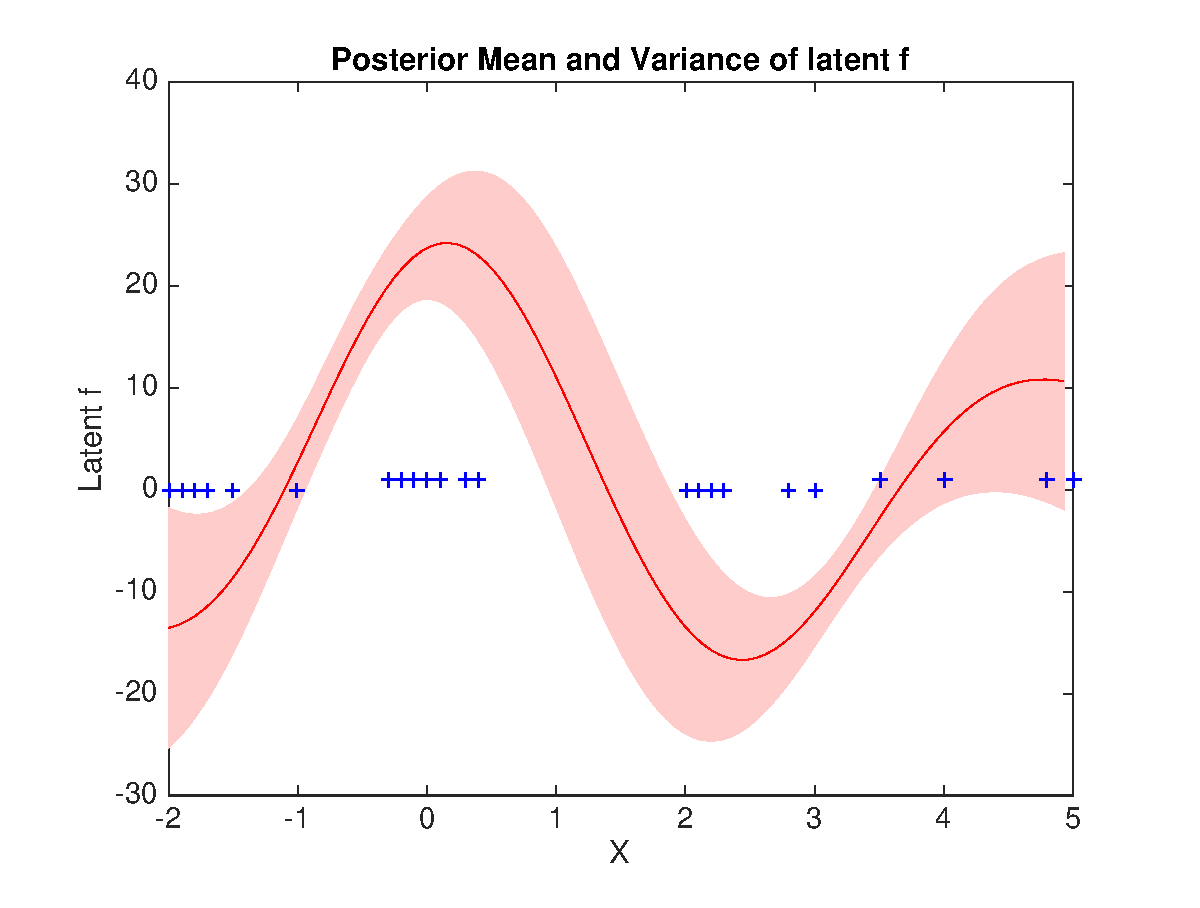
\includegraphics[scale=0.55]{classification_latent_f.eps}
\caption{Example plot of latent variable. Blue crosses are training points and red region is its variance. The variance now is never going to be zero because the latent function value is not observed directly. While in noise free regression, the exact value of output at training points is told.}
\end{figure}

\subsection{Maximising the Objective Function}
The objective function here is the log posterior $p(y|X,\theta) = \int p(y|f)p(f|X) df = \int \operatorname{exp}(\Psi(f)) df$ which can be obtained by using Laplace's approximation of $p(f|X,y)$ (Taylor expansion around $\hat{f}$)

\begin{equation}
p(y|X,\theta) \simeq q(y|X,\theta) = \exp(\Psi(\hat{f})) \int \operatorname{exp}(-\frac{1}{2}(f - \hat{f})A(f-f\hat{f})) df
\end{equation}
thus
\begin{equation}
\operatorname{log}q(y|X,\theta) = -\frac{1}{2}\hat{f}^TK^{-1}\hat{f} + \operatorname{log}p(y|\hat{f}) - \frac{1}{2}\operatorname{log}|B|
\label{eq:marg_likelihood_classification}
\end{equation}

where $|B| = |I_n + W^{\frac{1}{2}} K W^{\frac{1}{2}}|$ and $K$ is covariance defined by $\theta$. This is the final function we need to run optimisation on. 

\subsubsection{Sampling Methods for Hyperparameters}
In most of the cases, the objective functions are non-convex, which means that more than one set of initial hyperparameters has to be assigned as the starting points for optimisation. By running the optimisation algorithm starting from each set of them, the one gives the best result is chosen to be used for calculating the exact value of optimised hyperparameters. Following are two methods used for low number of hyperparameters (usually 1 or 2) and higher number of hyperparameters.


Uniform sampling is one of the most common and easily obtainable sampling method. Samples are simply drawn from sample space by dividing the sample space with the number of required samples and taking one in each subspaces (or more strictly, with equal distance between samples). This is usually an ideal sampling method for low dimensional problems where the number of dimensions will not largely increase the number of samples if we want to achieve the same number of sampling intervals in each dimension. 

\begin{figure}
\centering
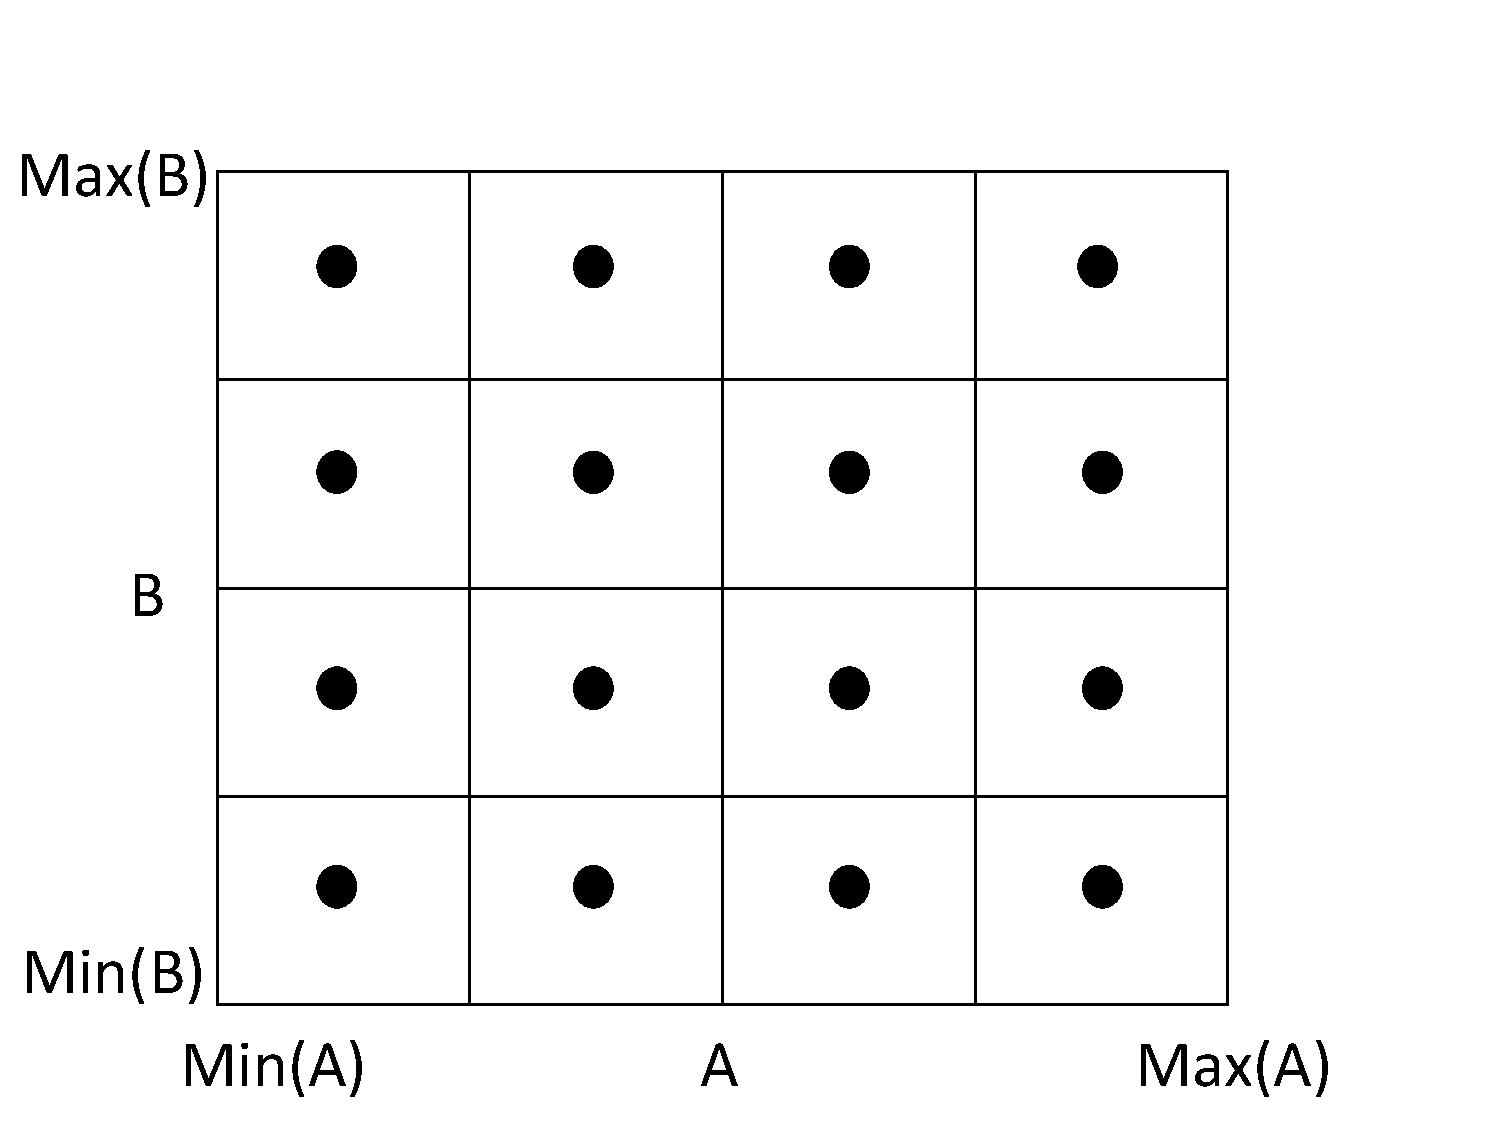
\includegraphics[scale=0.3]{Uniform_sampling.pdf}
\caption{A simple example of 2-dimensional uniform sampling with 4 sampling intervals in each dimension.}
\end{figure}


Latin Hypercube Sampling (LHS)\cite{mckay2000comparison} is commonly used for higher dimensional problems. If we want N samples from a one-dimensional variable, we can either uniformly take N points with equal distant from one another, or we can divide the sampling space into N equal intervals and take one sample from each interval. LHS is a simple extension from uniform sampling. When taking N samples from a M-dimensional variable, the sampling space of each dimension is divided into N equal intervals. Each interval is sampled once with the order of sampling being random. Then all the samples from M dimensions are combined to give N samples each has M dimensions. Each of the possible combinations of intervals forms a multi-dimensional region that sample could draw from, called a Latin square for two-dimensional sampling space and a Latin hypercube for higher dimensions. 

One advantage of LHS over random sampling is its uniformity. It ensures that samples are well-distributed in each dimension independently. While in random sampling, samples are generated without taking into account the previous samples, they results may be squeezed together, resulting in repeated optimisation results while leaving the other area blank. Non-linear function optimisation means that samples have to be well distributed. The more uniform the samples are, the more likely the global maximum could be found. Another important feature is that LHS does not require more samples for larger dimensions. In uniform sampling, a M-dimensional variable with N samples for each dimension means that N$\times$M samples will be drawn in order to cover the whole sampling space. Obviously for higher dimensional problems this is too time-consuming. For Gaussian process, the hyperparameters involved in optimisation include those used to define mean and covariance functions. The weightings of covariance function, each associated with a different input variable, are also treated as hyperparameters, high dimensional samples needs to be drawn, leading to a strong preference in Latin Hypercube Sampling.  

\begin{figure}
\begin{subfigure}{0.5\textwidth}
\centering
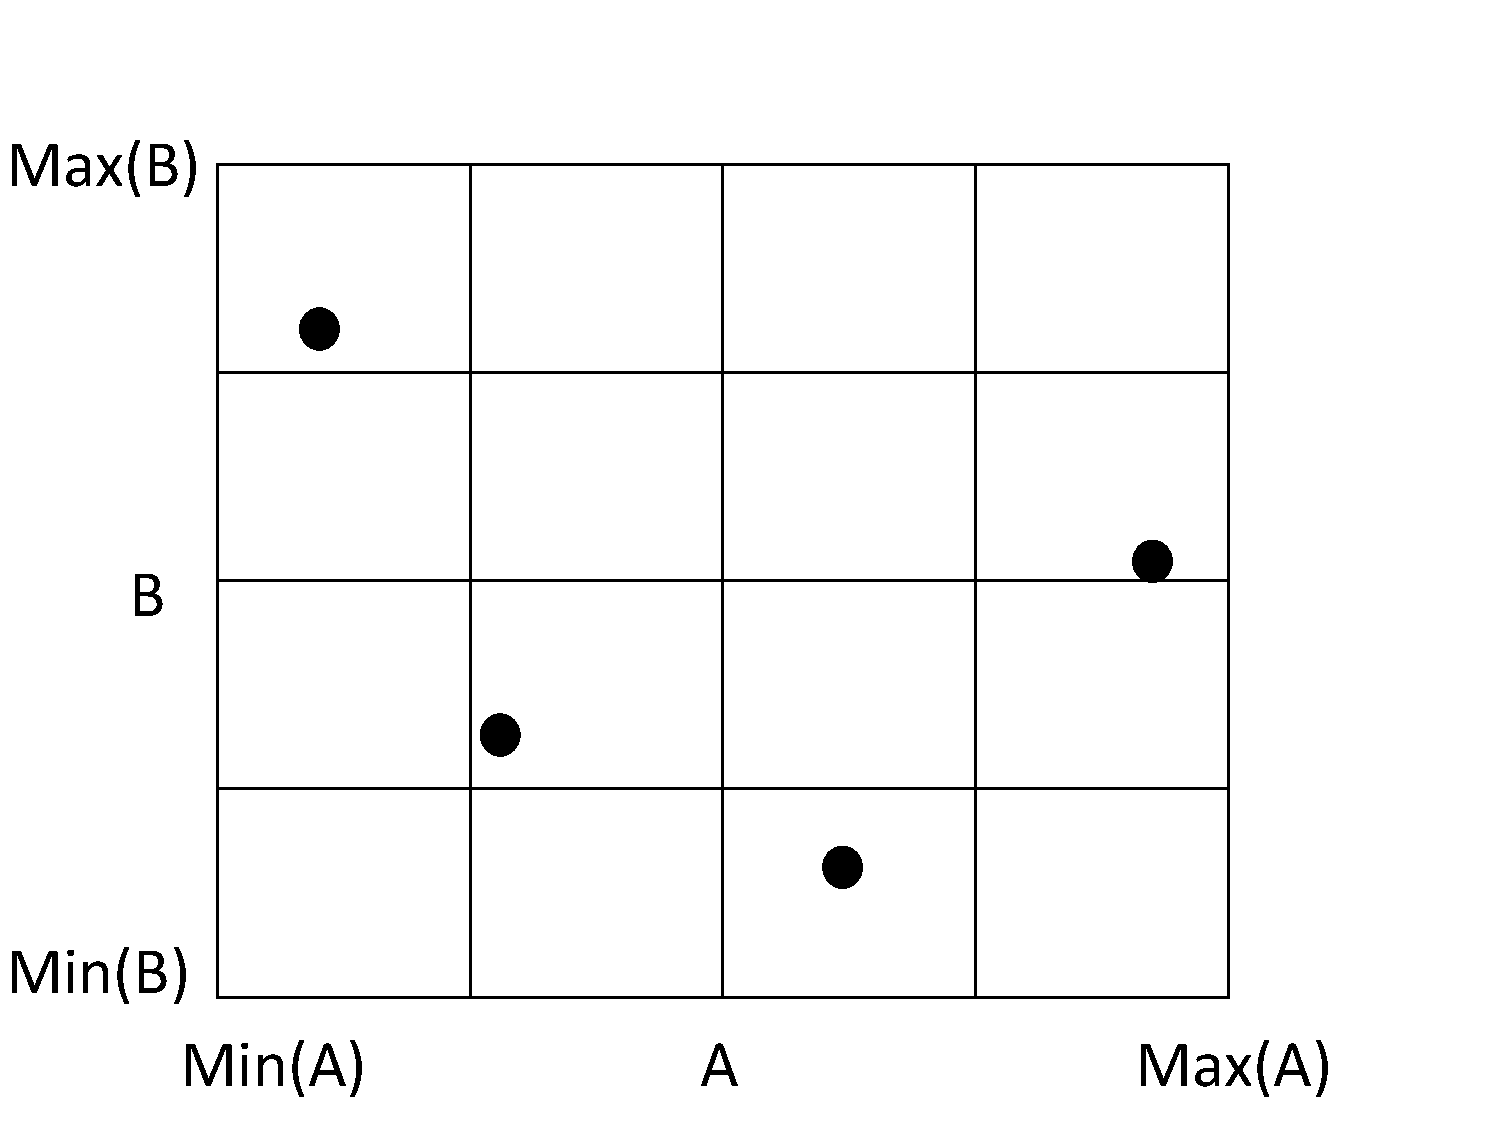
\includegraphics[scale = 0.3]{LHS.pdf}
\caption{Latin Hypercube Sampling}
\end{subfigure}
%\hspace*{0.02\textwidth}
\begin{subfigure}{0.5\textwidth}
\centering
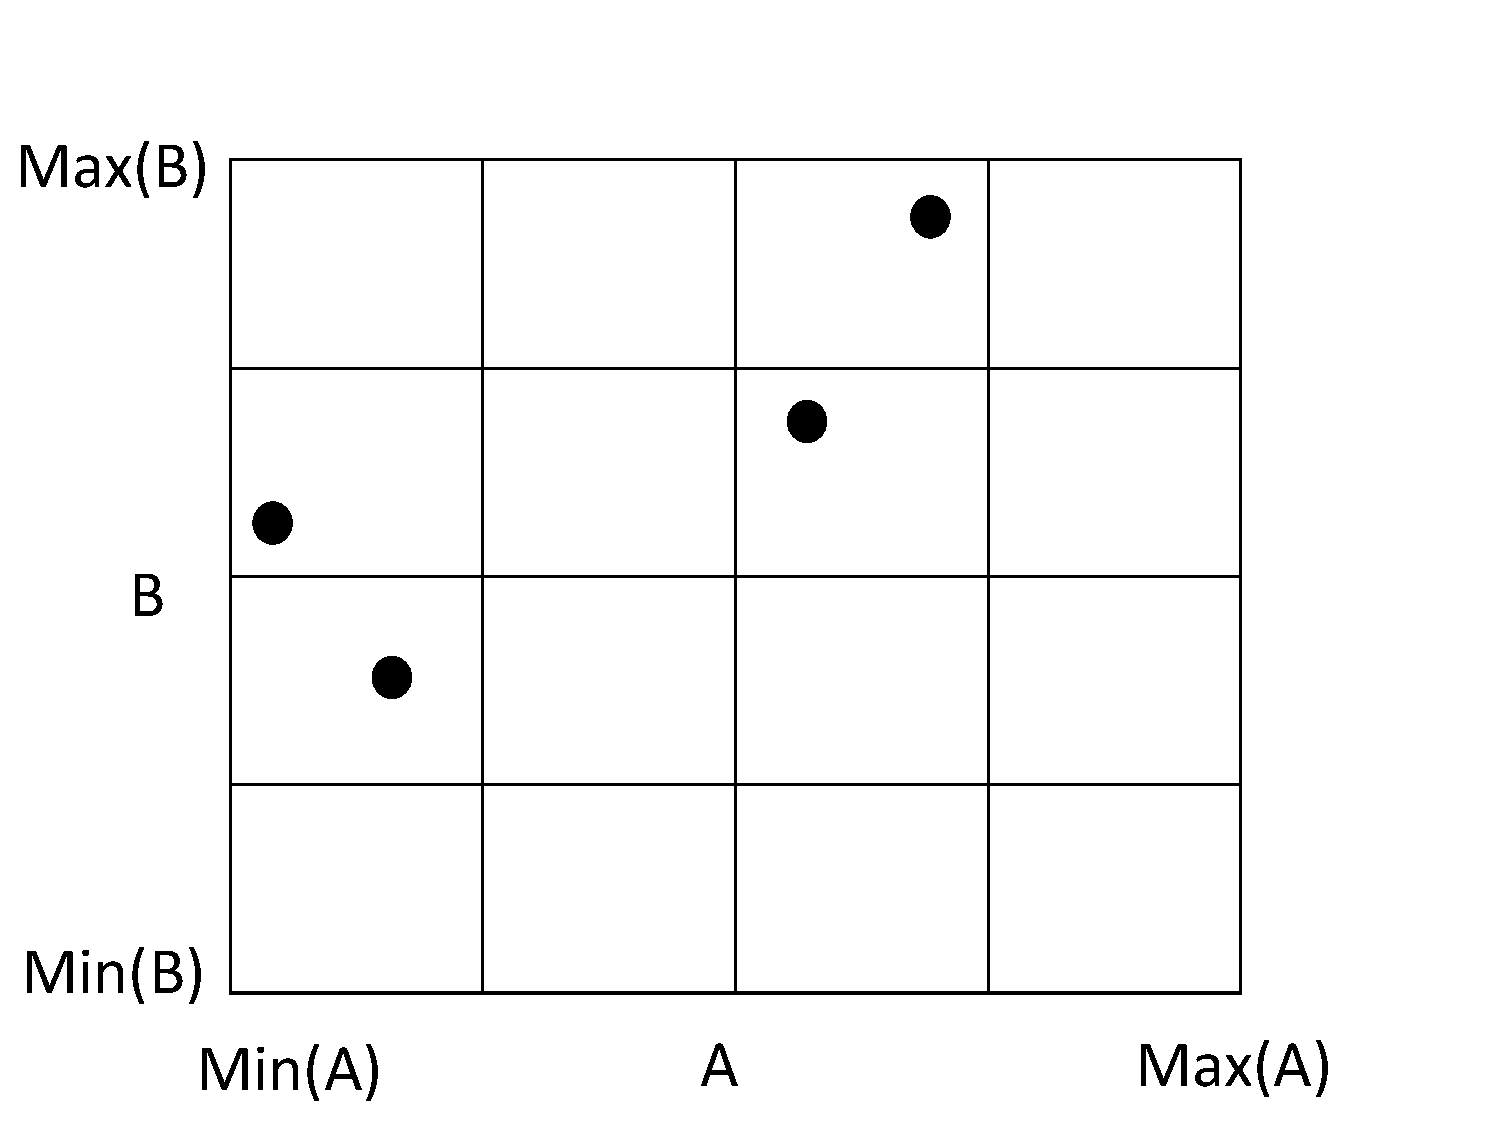
\includegraphics[scale = 0.3]{RS.pdf}
\caption{Random Sampling}
\end{subfigure}
\caption{Comparison between Latin Hypercube sampling and random sampling. Although Latin hypercube sampling may not represent the most variation overall ( can be improved by Orthogonal sampling), it gives a pretty good variability in each dimension. Random sampling does not secure any variability. }
\end{figure}



\subsubsection{Derivatives of Hyperparameters}

Again, as in regression, we need to find the gradient of likelihood w.r.t. all the hyperparameters we are trying to optimise. The case is slightly more difficult than regression as we introduced a latent variable $f$ and used Laplace's Approximation for likelihood itself. 

Since covariance matrix $K$ is a function of hyperparameters, therefore $\hat{f}$ and $W$ are implicit functions of hyperparameters. The derivative of equation (\ref{LaplaceApp}) is


\begin{equation}
\frac{\partial \operatorname{log}q(y|X,\theta)}{\partial \theta_i} = \frac{\partial \operatorname{log}q(y|X,\theta)}{\partial \theta_i}\bigg|_{explicit} + \sum_{i=1}^n \frac{\partial \operatorname{log}q(y|X,\theta)}{\partial \hat{f}_i}\frac{\partial \hat{f}_i}{\partial \theta_i}
\end{equation}

where


\begin{align} 
\label{eq:al1}
\frac{\partial \operatorname{log}q(y|X,\theta)}{\partial \theta_i}\bigg|_{\operatorname{explicit}} &= \frac{1}{2}\hat{f}^T K^{-1}\frac{\partial K}{\partial \theta_i}K^{-1}\hat{f} - \frac{1}{2}tr\Big((W^{-1}+K)^{-1}\frac{\partial K}{\partial \theta_i}\Big) \\ 
\label{eq:al2}
\frac{\partial \operatorname{log}q(y|X,\theta)}{\partial \hat{f}_i} &= -\frac{1}{2} \big[(K^{-1}+W)^{-1}\big]_{ii}\frac{\partial^3}{\partial f_i^3}\operatorname{log}p(y|\hat{f})
\end{align}



\subsection{Predictive Probability}
Predictive mean can be decided under Laplace's approximation by combining the prediction in regression eq. (\ref{predictive_mean_noise_free}) with eq. (\ref{optimised_f})

\begin{equation}
\label{predictive_mean_classification}
\mathbb{E}[f_\ast|X,y,x_\ast] = K(X_\ast, X)K(X, X)^{-1}\hat{f} = K(X_\ast, X) \nabla\operatorname{log}p(y|\hat{f}) 
\end{equation}

Predictive variance consists of two terms: one from $f_\ast$ given $f$, the other from our estimation of $f$

\begin{equation}
\label{predictive_var_classification}
\mathbb{V}[f_\ast|X,y,x_\ast] = \mathbb{E}[(f_\ast - \mathbb{E}[f_\ast|X,y,x_\ast])^2] + \mathbb{E}[(\mathbb{E}[f_\ast|X,x_\ast,f] - \mathbb{E}[f_\ast|X,y,x_\ast])^2]
\end{equation}

using the matrix inversion lemma\cite{woodbury1950inverting} we get

\begin{equation}
\mathbb{V}[f_\ast|X,y,x_\ast] = K(x_\ast,x_\ast) - K(x_\ast,X)(K(X,X) + W^{-1})^{-1}K(X,x_\ast)
\end{equation}

Predictive probability the new output belong to class 1 is then computed by eq. (\ref{predictive_probability}) except that the distribution of $f_\ast$ is now the result of Laplace's approximation with mean and variance as stated above. 

\begin{equation}
\bar{\pi}_* \triangleq p(y_* = +1|X,y,x_*) = \int \sigma (f_*)q(f_*|X,y,x_*) df_*
\end{equation}

One may argue that expectation of the prediction could be simply equal to the sigmoidal mean of $f_*$. These are actually two different things because of the non-linearity of sigmoid function, the first is averaged probability $E[\pi_*|X,y,x_*]$ while the later one is MAP prediction $\sigma (E[f_*|y])$. Although the final class labels assigned are the same for both cases, only the averaged probability gives the statistically correct results. 

\begin{figure}[!htb]

\begin{subfigure}{0.48\textwidth}
\centering
	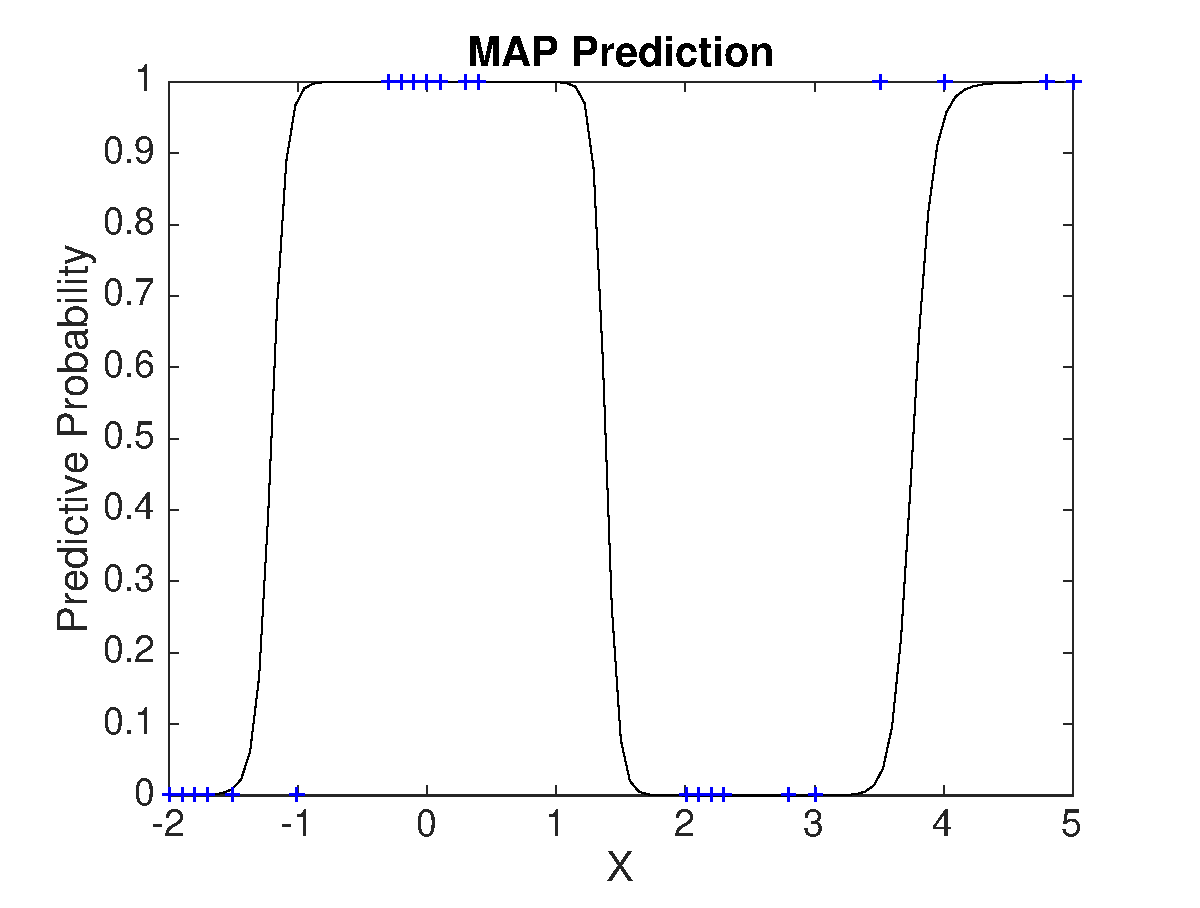
\includegraphics[scale = 0.42]{classification_MAP.eps}
	\caption{}
\end{subfigure}%
\hspace*{0.03\textwidth}
\begin{subfigure}{0.48\textwidth}
\centering
	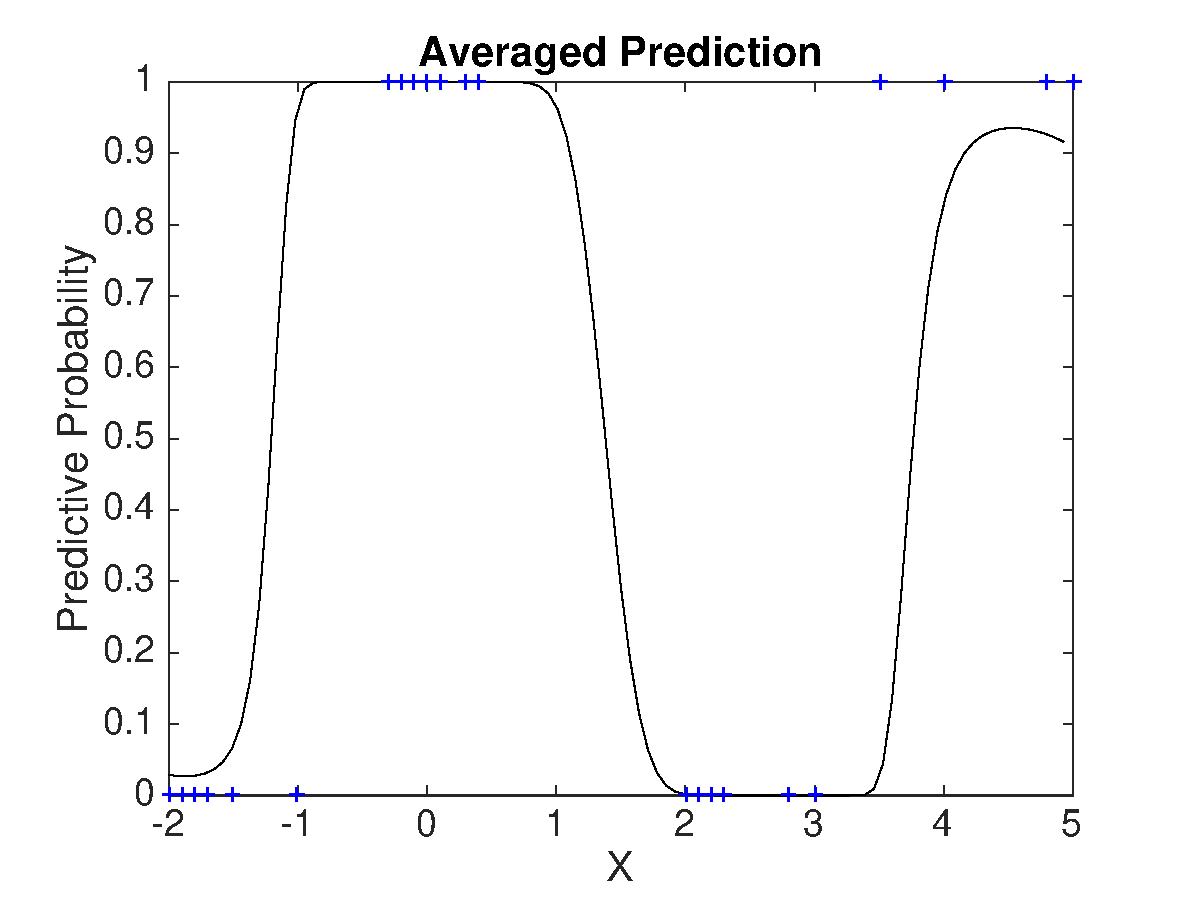
\includegraphics[scale = 0.42]{classification_ave.eps}
	\caption{}
\end{subfigure}

\caption{(a) the MAP prediction. (b) the averaged probability prediction. Blue crosses are training points (class label 1 and -1 but marked as 1 and 0 for better display). The MAP prediction goes to the extremes quicker while the averaged probability is more moderate and tend to be affected by adjacent points}

\end{figure}

\newpage
\section{Data Preprocessing}
\rhead{Data Preprocessing}
\label{sec:preprocessing}
Sometimes only the useful information is wanted when data is noisy or redundant. This can be achieved by data preprocessing. It has a few advantages. First, for high dimensional data, computation time is essential. Reducing the redundant information can largely save computation time. Second, less redundant information means it is easier for your algorithm to find the true pattern behind data. 

\subsection{Principal Component Analysis}
Principal Component Analysis (PCA) is a statistical tool for dimensionality reduction. It tries to identify the subspace in which the data approximately lies. It transforms the original data into orthogonal components in descending order of their corresponding variances\cite{jolliffe2002principal} by eigenvalue decomposition or singular value decomposition\cite{golub1965calculating}. The resulting number of principal components is always equal or less than the original number of dimensions. This can be intuitively explained by the orthogonality of the principal components. Orthogonality means that components are uncorrelated and there are no redundant information between them. Therefore less number of components are needed to represent the data. 

The steps for using PCA is very simple: First, normalise the data in each dimension. Next, put it through singular value decomposition. Lastly, cut off all the components with variances less than a threshold. Threshold value depends on how much variances user wants  to retained. PCA is widely used in supervised machine learning for faster computation and better knowledge discovery. When dropping the components with less variances, it is equivalently to give up those unimportant features that may had affected the resulting model.  

 
\subsection{Normalisation}
Since PCA is sensitive to the relative scaling of the original variables, normalisation\cite{kotsiantis2006data} is needed before applying PCA\cite{PCA_AN}. There are three common methods for normalisation: simple rescaling, per-example mean subtraction, and feature standardization. Simple rescaling are usually used in image processing when pixel value is rescaled from [0,255] to [0,1] by dividing 255 on each element. Per-example mean subtraction is suitable for stationary data that the statistics for each feature dimension is the same. Simply subtracting the mean value of each instance would be enough. The third one, feature standardization, is the most common method for normalisation. It is achieved by first subtract the mean of each dimension from that dimension. Then, each feature dimension is divided by the standard deviation of that dimension. The process makes each dimension to have zero mean and unit variance. With all dimensions having the same scale, PCA can then be applied.



\chapter{GP Classification for Employment Prediction}
\rhead{GP for Employment}
\label{GP_for_employment}
To integrate Gaussian process classification into the prediction of occupational automatability, we first define the occupational features as the input and the probability of computerisation as the output. The basic idea is first to train a classifier based on labeled occupational features. Then the classifier is used to make prediction on occupations with unknown labels, or in other words, to determine the probability of any unknown occupation belonging to class '1'. Here class '1' means the occupation is automatable, and class '0' means it is not automatable. The same class notation will be used through the project.  
  

\begin{figure}[htb]
\centering
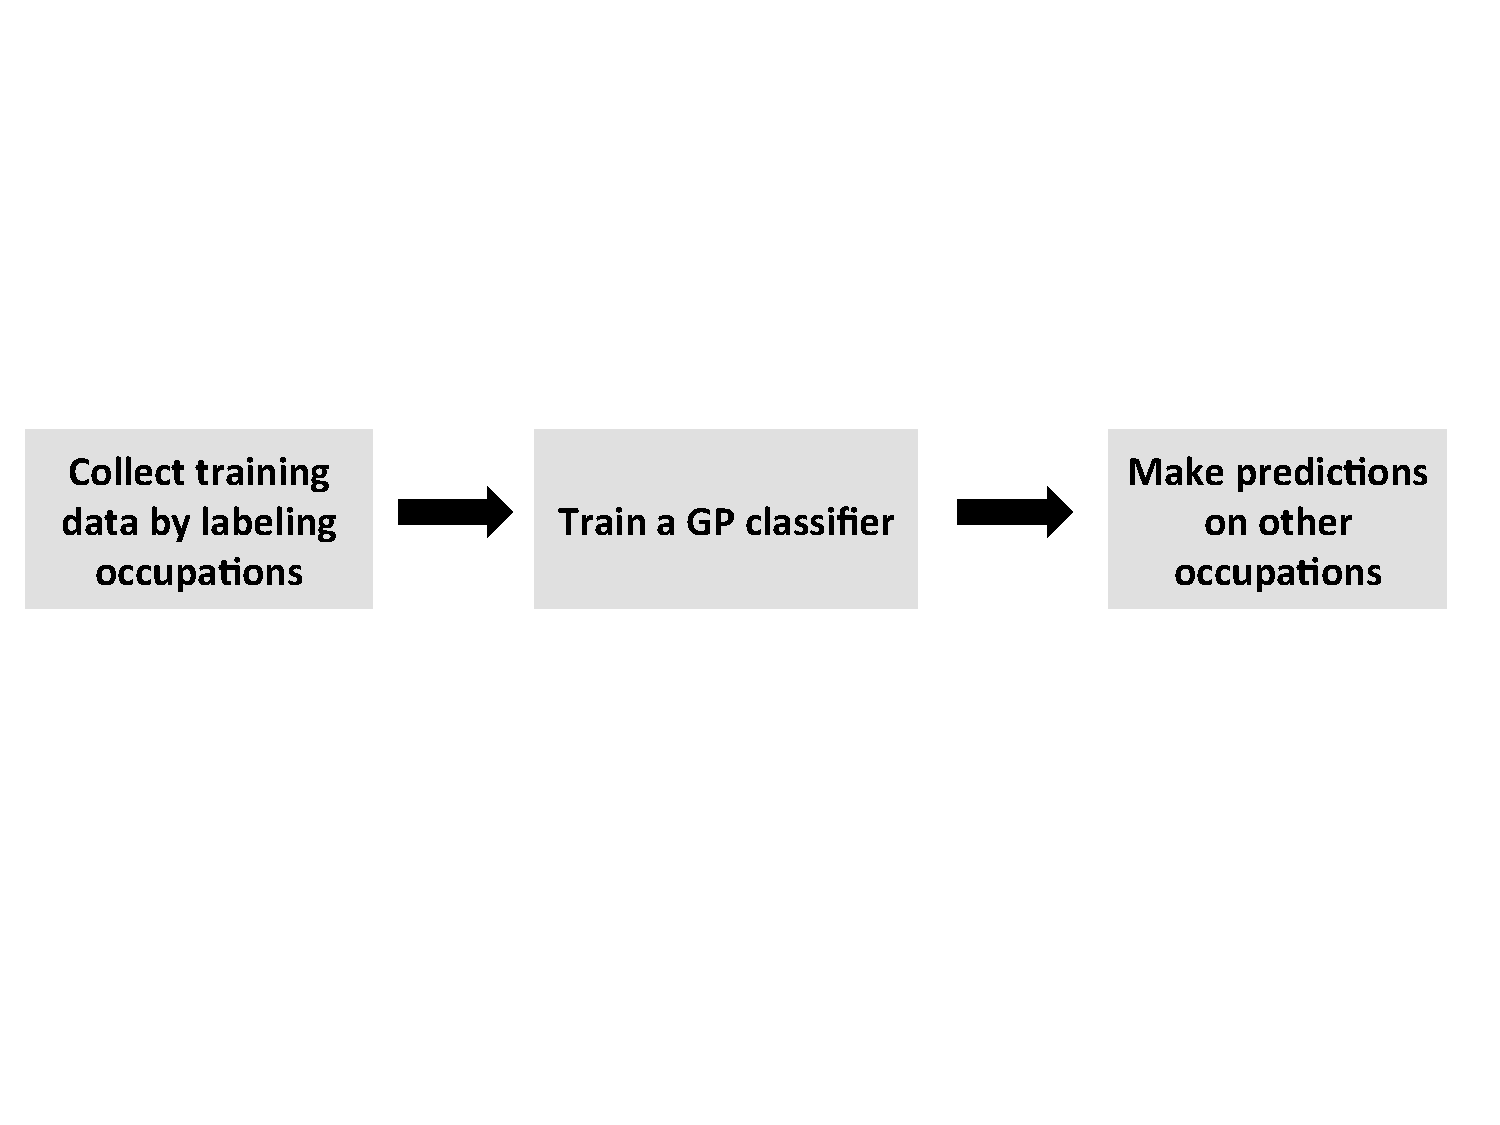
\includegraphics[scale=0.6]{prediction_flow.pdf}
\caption{A flow chart for how predictions are made}
\label{fig:flow}
\end{figure}
 

\section{Performance Measurement} 
There are two possible measurements for predictive accuracy: marginal likelihood and Receiver Operating Characteristic (ROC) curve. One is marginal likelihood calculated in equation \ref{eq:marg_likelihood_classification}. It is also a measure for choosing hyperparameters. The higher (less negative) its value is, the better the performance. Both likelihood and ROC are computed on verification set rather than training set. How these two sets are formed will be discussed later. 

The other important measure commonly used in binary classifier, ROC \cite{hanley1982meaning}\cite{bradley1997use}, plots the true positive rate against the false positive rate.The area under the ROC curve (AUC) gives the probability that the classifier gives the right answer for positive classes. A random classifier would score an AUC of 0.5 while a perfect classifier would give the AUC of 1. 

There are possibilities of model over-fitting or under-fitting. Whether they would occur depends on the value of hyperparameters. A simple illustration of over-fitting and under-fitting in 1D Gaussian process is shown in Figure \ref{fig:overfitting}. In the upper left graph, when length scale is small, the model function tries to fit too much details including the unwanted noise. While in the upper right graph, when length scale is too large, the model would only describe a general trend which is not very useful if more information is wanted. The best model is the intermediate state where only the appropriate curvatures are preserved. 

\begin{figure}[!htb]

\begin{subfigure}{0.48\textwidth}
\centering
	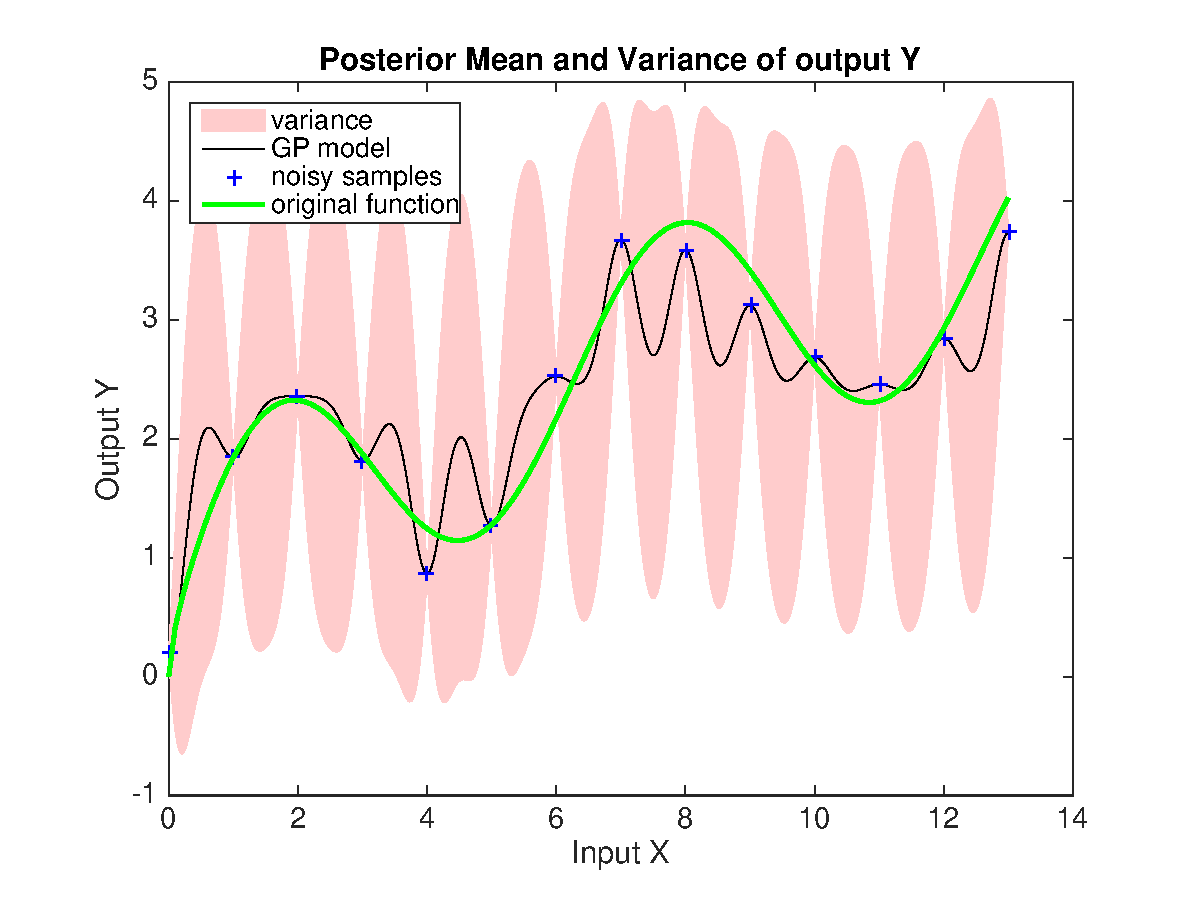
\includegraphics[scale = 0.4]{overfit.eps}
	\caption{over-fitting, $l$ = 0.25}
\end{subfigure}%
\hspace*{0.05\textwidth}
\begin{subfigure}{0.48\textwidth}
\centering
	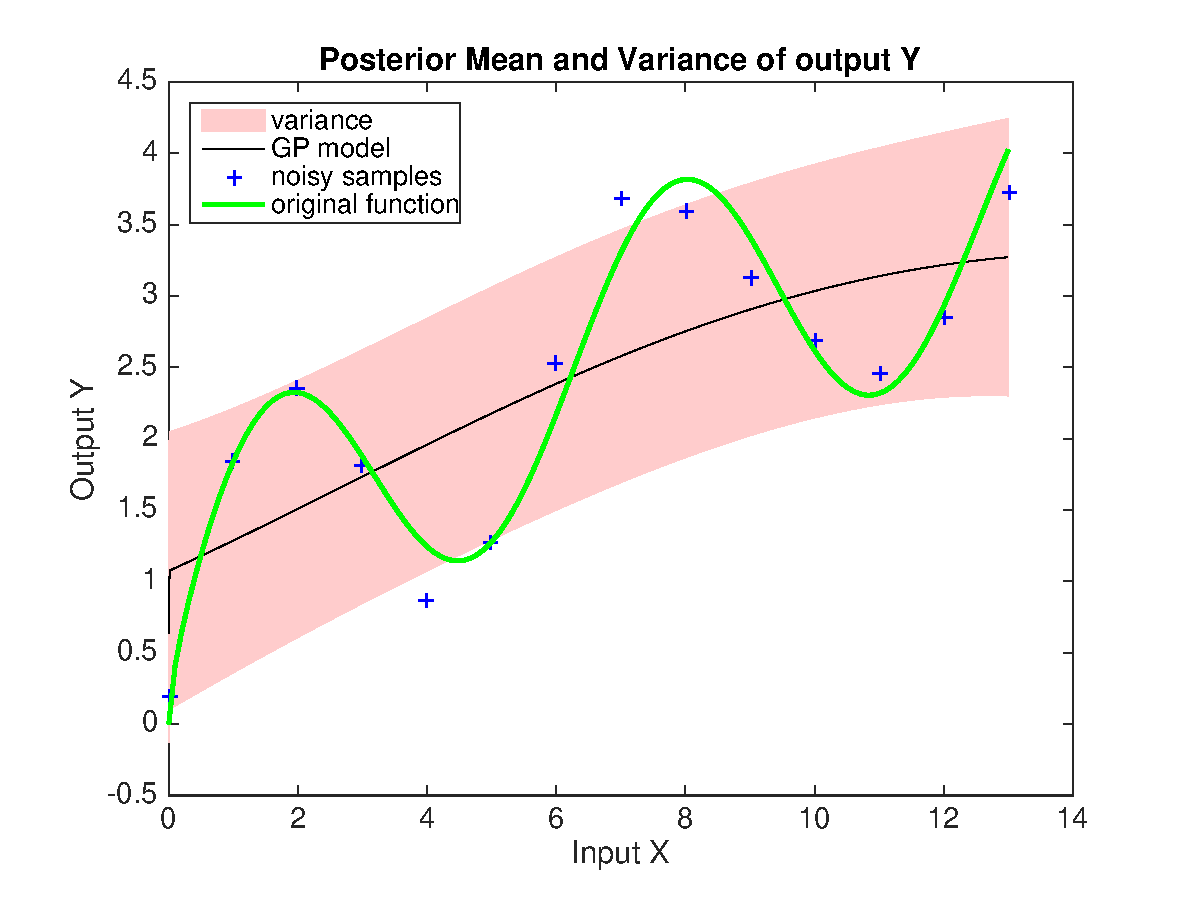
\includegraphics[scale = 0.4]{underfit.eps}
	\caption{under-fitting, $l$ = 12}
\end{subfigure}\\

\hspace*{0.25\textwidth}
\begin{subfigure}{0.48\textwidth}
\centering
	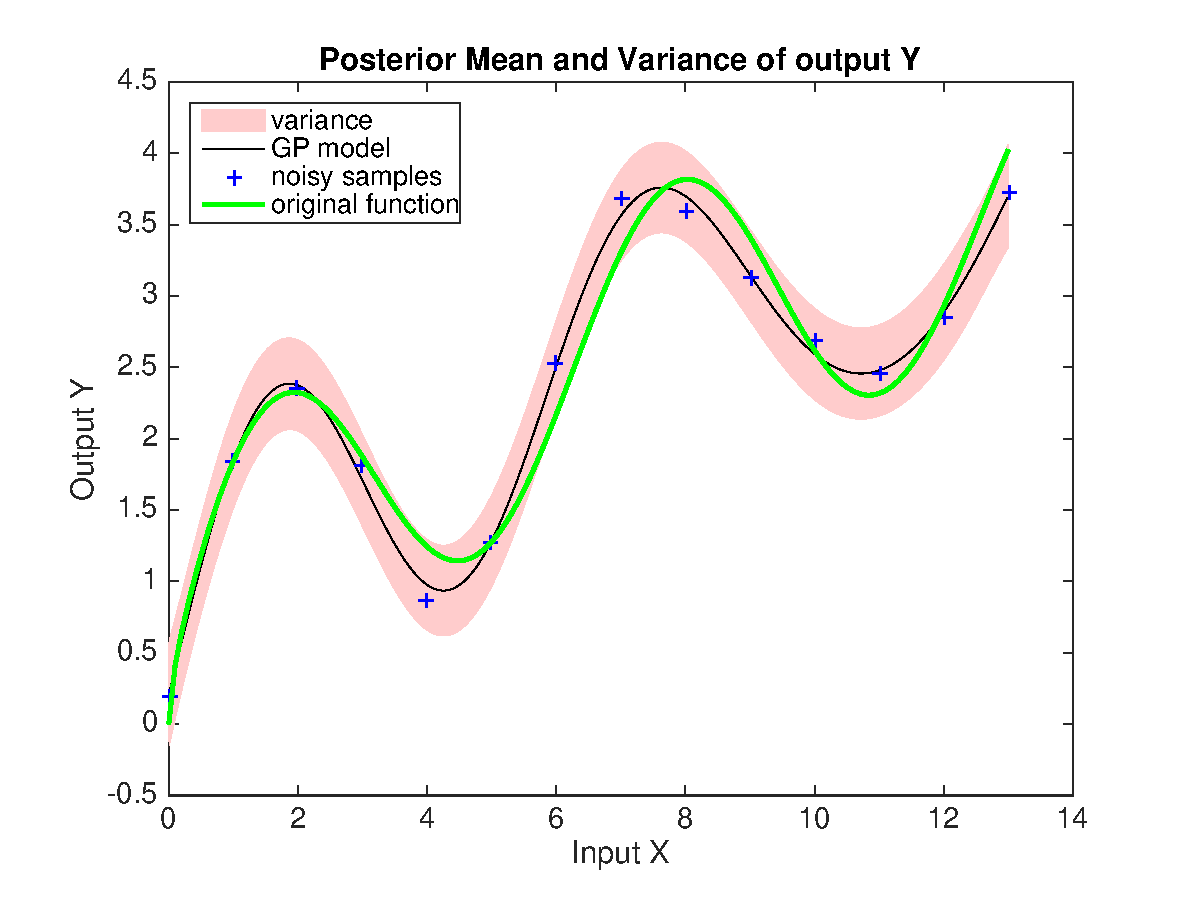
\includegraphics[scale = 0.4]{fit.eps}
	\caption{$l$ = 2}
\end{subfigure}



\caption{(a) When lengthscale get small, it tries to fit the noise-corrupted details (b) If length-scale is constrained to be large, it concentrates on large scale smoothness (c) An appropriate model in this case should pay attention to detail but not forgetting the overall smoothness. Green curve is the original function from which noisy samples (blue crosses) are generated. Black curve is the resulting GP model.}

\label{fig:overfitting}
\end{figure}

In order to verify that the classifier is working correctly, i.e. no over-fitting or under-fitting is happening, AUC is computed by dividing the training data into a testing group and a training group with equal number of members each. The model hyperparameters trained from the training group are used for predicting the testing group labels. Then the result of testing group is compared with its true class labels to generate the ROC curve. A typical ROC curve in this problem would look like figure \ref{fig:ROC}. The final model for predicting all occupations are trained on the whole training set which includes the training group and testing group. One thing to notice is that a good algorithm learns the trend from training data while not fitting the noise. Noise can be introduced when the feature variables are noisy or the labels are not 100\% correct. An ideal model should be able to identify and correct the mistaken labels therefore would not necessary give the lowest training error or the best AUC.


\begin{figure}[!htb]
\centering
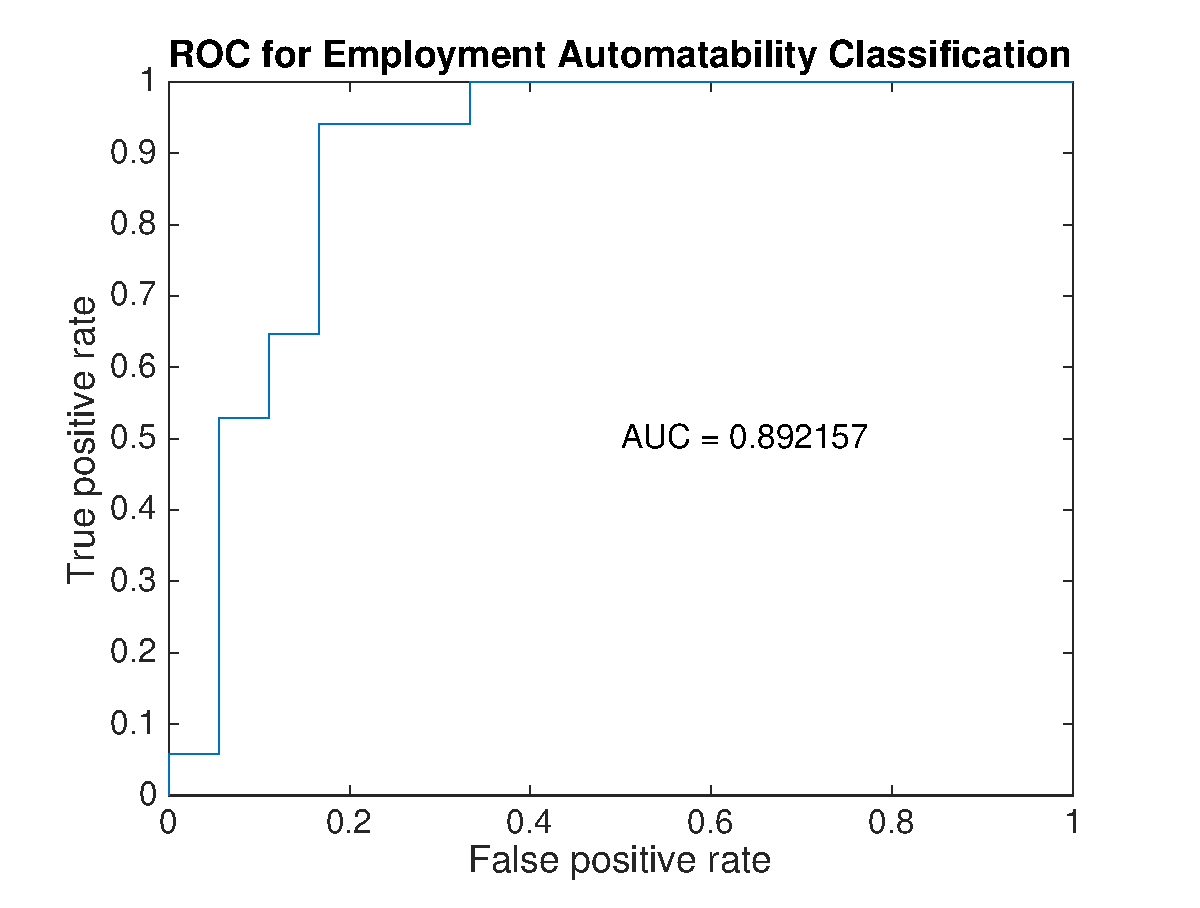
\includegraphics[scale=0.5]{ROC1.eps}
\caption{A typical ROC curve plotted with 35 training instances. }
\label{fig:ROC}
\end{figure}



\newpage
\section{The 2010 data}%% story telling mode!!!! 
The occupational task descriptions are obtained from the 2010 version of O*NET -- an online platform providing detailed descriptions for jobs. Hand-labelled training data with 33 occupations labelled '0'(not automatable) and 37 labelled '1'(fully automatable) are prepared. A job is defined as automatable if all tasks involved in that job can be performed by computer-controlled equipment. More details about how the training data is determined can be found in the work of Frey \& Osborne\cite{frey2013future}.  

Nine features, falling into three categories -- social intelligence, creative intelligence, and perception and manipulation, are believed to be bottlenecks of computerisation. They  are important factors that affect automatability in terms of the intelligence required to perform a job. Hence concatenating these nine features of each occupation into a feature vector would give us the input of the classification algorithm. Using the feature vector and class label for each occupation in the training set, the probability of any other occupation with unseen feature vector can be computed by estimating a latent function and then mapped into a probability value between 0 and 1. Note the probability computed is only suitable for the near future since the labels are based on current technology capability.

As stated in section \ref{sigmoid function}, any type of sigmoid function could be used in this mapping. Two most common types of sigmoid funcion is discussed here: probit\footnote{Also know as cumulative Gaussian function} and logistic function. If using each of them for training and prediction, we could get two sets of performance measurements. Marginal likelihood and AUC are computed on validation set for each sigmoid function. In Table \ref{tab:sigmoid} we could see that probit function outperforms logistic function in both likelihood and AUC. Hence probit function is chosen as the better sigmoid function for this particular problem. 

Squared exponential is used as the covariance function since the output is not expected to have any periodicity but a general smoothness would be helpful (occupations with similar feature variables should have a similar probability of being automated). MinConf\cite{minConf} is used for fast optimisation on multivariate objective function subject to simple constraints on the parameters. The hyperparameters are constrained within certain ranges for numerical stability. 

\renewcommand{\arraystretch}{2}  %table line width
\begin{table}[!htb]
\centering
\begin{tabular}{?c|c|l?}
\thickhline
Performance & Probit & Logistic \\ \hline
Likelihood  & -30.86 & -31.80   \\
AUC         & 0.92   & 0.85     \\ \thickhline
\end{tabular}
\caption{Performance comparison between probit function and logistic function}
\label{tab:sigmoid}
\end{table}



The results are shown in Figure \ref{fig:category2010}. In stead of plotting original variables against the probability of computerisation, the graphs are generated by plotting the categorical score against probability. The value for each category is calculated by adding up all variables in that category. The categorical plots show a clear trend in automatability. 


\begin{figure}[!htb]
\centering
\begin{subfigure}{0.55\textwidth}
\centering
	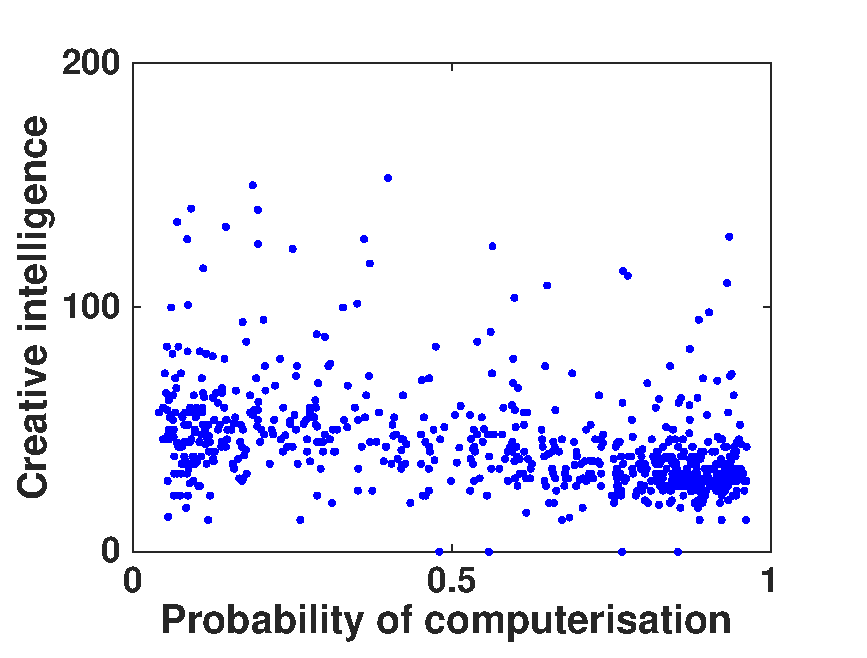
\includegraphics[scale = 0.5]{creative_intelligence.eps}
\end{subfigure} \\
\begin{subfigure}{0.55\textwidth}
\centering
	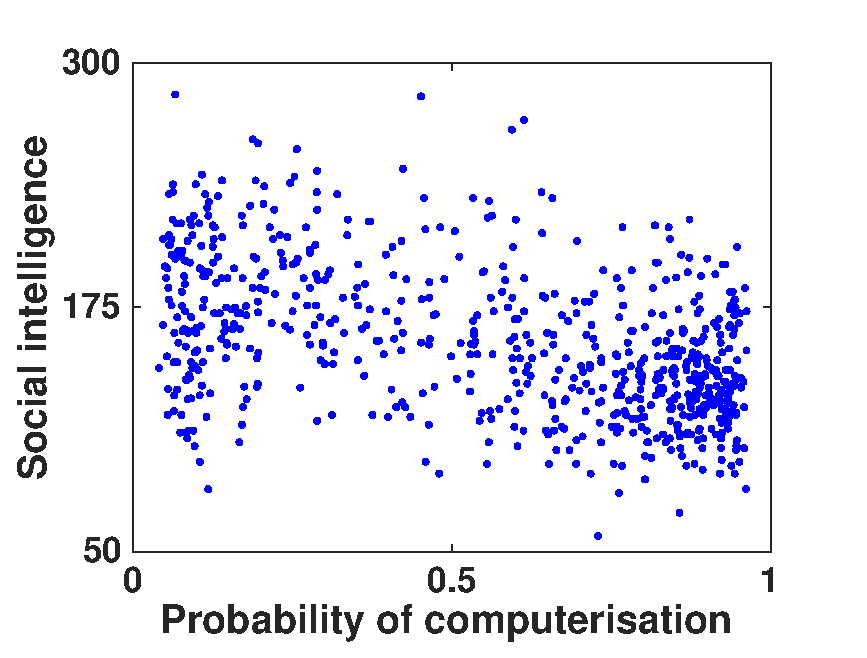
\includegraphics[scale = 0.5]{social_intelligence.eps}
\end{subfigure}\\

\begin{subfigure}{0.55\textwidth}
\centering
	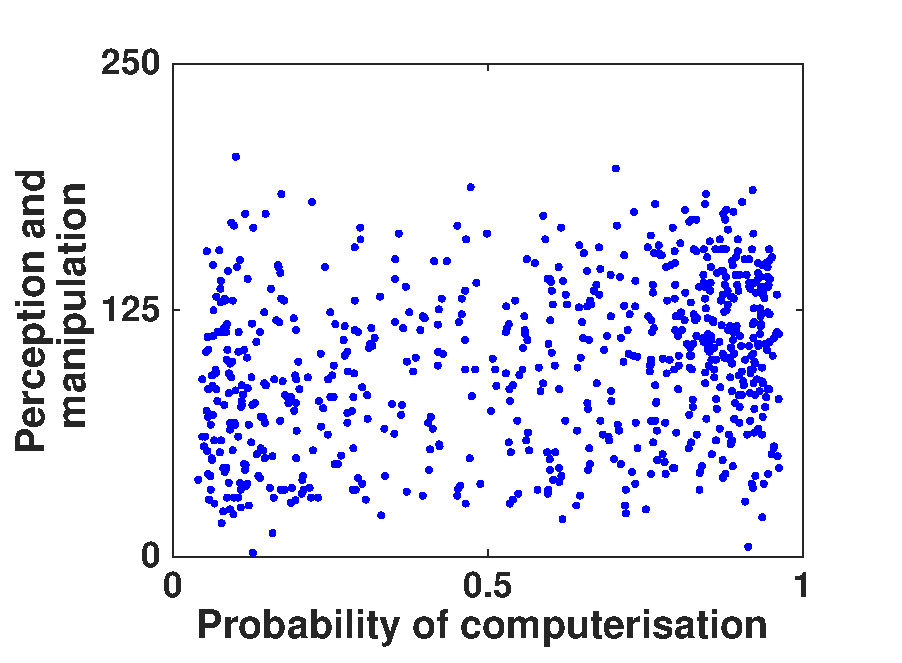
\includegraphics[scale = 0.5]{perception_and_manipulation.eps}
\end{subfigure}


\caption{The occupational category as a function of probability of computerisation. Each point represents an occupation. The value for each category is computed by adding up all variables within that category but the input for the algorithm is still nine variables.}
\label{fig:category2010}
\end{figure}

Both creative intelligence and social intelligence have a negative effect on probability of computerisation. High values in these variables indicate a lower risk of being automated. On the other hand, occupations with high value in variables of perception and manipulation tend to have a higher risk. For example, 'Mental Health Counselors' needs a high level of social perspectives such as persuasion, have a probability as low as 0.048. However, machine operators such as 'Shoe Machine Operators and Tenders' require a relatively higher level of manual dexterity, has a high probability of 0.95. Probability of other occupations can be checked in Appendix \ref{App:results_all}.

It is not hard to tell that occupations involving abstract and creative tasks are not likely to be substituted by machines, at least not now, not on a large scale. Although, it does not mean that jobs requiring high creative intelligence and social intelligence will never be automated, it does indicates that these substitution is not happening in the near future given current technology. 

However, we should always be aware that automation in these areas could happen when their engineering bottlenecks are broken. At that time, there is no reason for automation not to happen when machines can just perform these tasks as well as human and even at a lower cost. This is exactly what happened after the Great Recession -- companies preferred to buy more equipments than hire more employees. It was believed to be the fundamental cause of the slow recovery of labor force market after the recession\cite{brynjolfsson2012race} and it could also be the cause of the next job loss.








\newpage
\section{The 1980 data}
Occupational data from previous work\cite{david2001skill}, including skills required in each occupation in 1980, is used to compute the automatability in 1980. In total, there are 26 input variables for each occupation such as spatial aptitude, clerical perception, and finger dexterity etc. All of these variables are chosen from \textit{Handbook for Analyzing Jobs}\footnotemark. 

\footnotetext{U. S. Department of Labor, Manpower Administration, Handbook for Analyzing Jobs (Washington, DC, 1972)}

Before experiment starts, training labels from the 2010 experiment are transferred to 1980 occupations via crosswalk files\cite{SOC2010_2000},\cite{SOC2000_OCC}, and\cite{OCC2000_1990}, giving 58 labels on the new data. Here it is assumed that the task breakdown of jobs has not changed too much from 1980 to 2010. Directly transferring the labels to the 1980 data also means that the impact of 2013 technology is introduced in the 1980 result. Therefore it is reasonable to expect that the 2013 technology would be able to automate more simpler jobs no longer exist today but available in 1980. 

In order to get better results on classification and saving computation time, principal component analysis (PCA) is used to reduce the dimensionality of feature vector. First the data is normalised by setting each dimension to zero mean and unit variance (Section \ref{sec:preprocessing}). Then applying PCA on the 26 dimensional input. 19 components are remained when 98\% of variances are preserved. The reduced feature vectors are then used as the input variables for computerisation prediction. Again, marginal likelihood and the AUC of validation set when using and not using PCA in the preprocessing step are compared to show whether PCA has improved the performance (Table \ref{tab:PCA}). The result shows that PCA does improve both likelihood and AUC. This is not a surprise since 26 variables are very likely to introduce some degree of noise and PCA can help removing the noise. \\


\begin{table}[]
\centering
\begin{tabular}{?c|c|l?}
\thickhline
Performance & no PCA & with PCA \\ \hline
Likelihood  & -35.99 & -30.65   \\
AUC         & 0.75   & 0.87     \\ \thickhline
\end{tabular}
\caption{Performance with and without PCA}
\label{tab:PCA}
\end{table}


Only five measurements are analysed as representatives for five types of task\cite{david2001skill}. They are routine cognitive, routine manual, non-routine analytical, non-routine interactive, and non-routine manual tasks. A task is defined as 'routine' if it can be accomplished by machine following explicit rules that can be programmed. Many rule-based tasks, such as monitoring the amount of sulphur dioxide in gas emitted by thermal power station, belong to this category. Non-routine tasks are those that can not be programmed in code line by line and therefore are well understood by computers. Another categorization is manual or cognitive. Manual tasks involves physical activities while cognitive tasks involves knowledge works. Cognitive tasks can further be categorised into analytical or interactive, depending on whether it needs mathematical skills or not. 

Although the input variables for 2010 and 1980 are both about the level of intelligence required to perform a job, their analysis focus on different perspectives. Previously, the study focused on the relation between score of intelligence and probability. This time, the score of intelligence is used as representatives for different tasks. Certainly there is a  correspondence between these two representations. Social intelligence is often required in non-routine interactive tasks while perception and manipulation are mostly performed in either routine or non-routine manual tasks. Similar trends would be expected for corresponding categories. Figure \ref{fig:1980} are the probability plot for all five tasks. The score of each task is calculated as the percentage of the sum of all five task scores. As expected, high level of non-routine interactive tasks means lower probability of computerisation. High level of routine and non-routine manual tasks gives higher risk for computerisation.

\begin{figure}[!htb]

\begin{subfigure}{0.5\textwidth}
\centering
	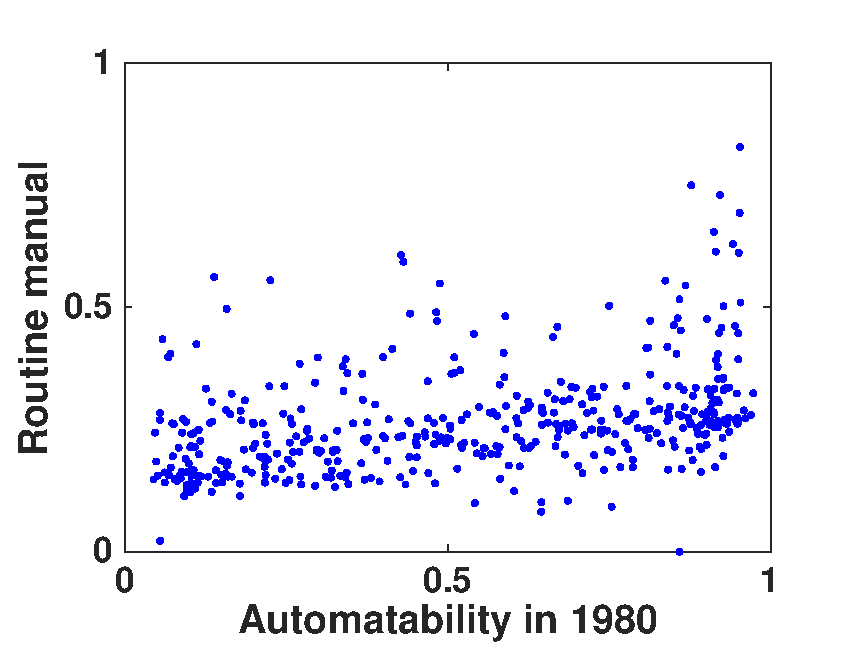
\includegraphics[scale = 0.5]{routine_manual.eps}
\end{subfigure}%
%\hspace*{0.05\textwidth}
\begin{subfigure}{0.5\textwidth}
\centering
	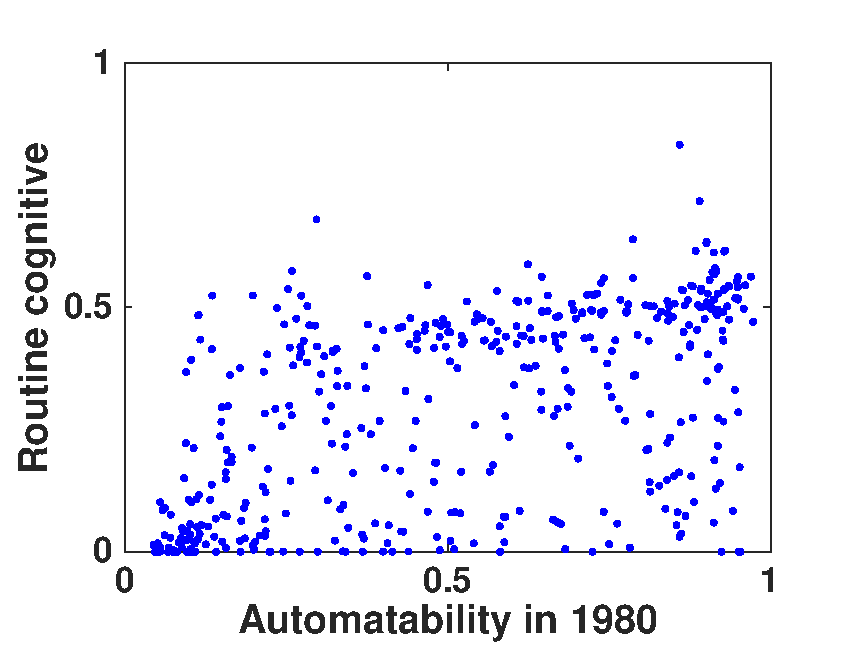
\includegraphics[scale = 0.5]{routine_cognitive.eps}
\end{subfigure}\\

\begin{subfigure}{0.5\textwidth}
\centering
	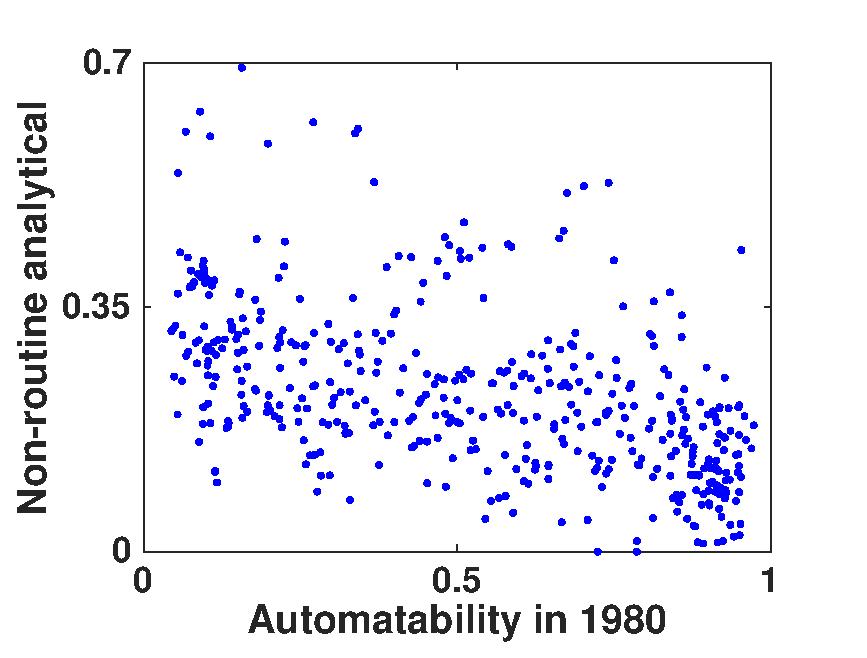
\includegraphics[scale = 0.5]{non-routine_analytical.eps}
\end{subfigure}%
\begin{subfigure}{0.5\textwidth}
\centering
	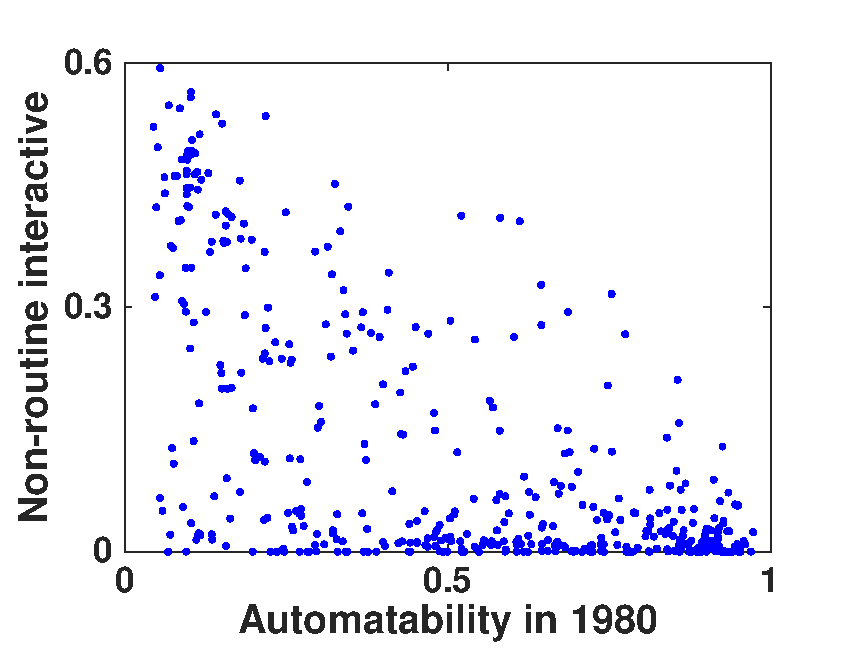
\includegraphics[scale = 0.5]{non-routine_interactive.eps}
\end{subfigure}\\\centering
\begin{subfigure}{0.5\textwidth}
\centering
	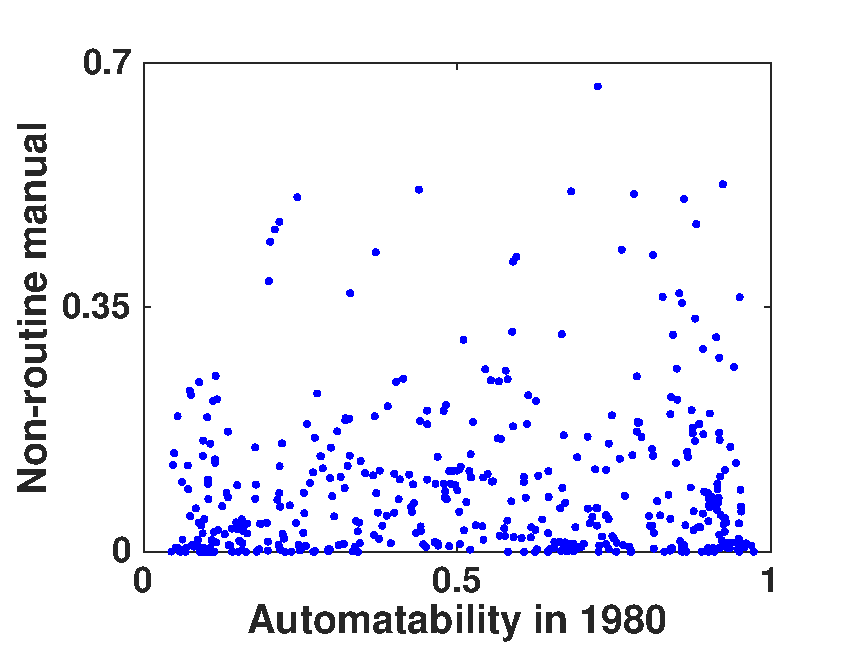
\includegraphics[scale = 0.5]{non-routine_manual.eps}
\end{subfigure}

\caption{The task measurements in 1980 vs. \\probability of computerisation.}
\label{fig:1980}
\end{figure}


One interesting thing to notice is that the trend for non-routine manual task is more similar to those of routine tasks. In the 20th century, computerisation is limited within routine tasks that can be performed by following explicit rules. Recent developments in artificial intelligence makes non-routine tasks involving non-rule-based activities such as pattern recognition also become computerisable. This is why non-routine manual task behaves like routine tasks. An example occupation rich in non-routine manual tasks would be drivers. Traditionally, driving a car is treated as a fairly difficult task for machine to complete. Now self-driving car is believed to be undoubtedly the next revolution in car industry. Similar things are happening in other areas. All of them contribute to the change of computerisation and as a result shift in job market.



\begin{figure}[htb]

\begin{subfigure}{0.48\textwidth}
\centering
	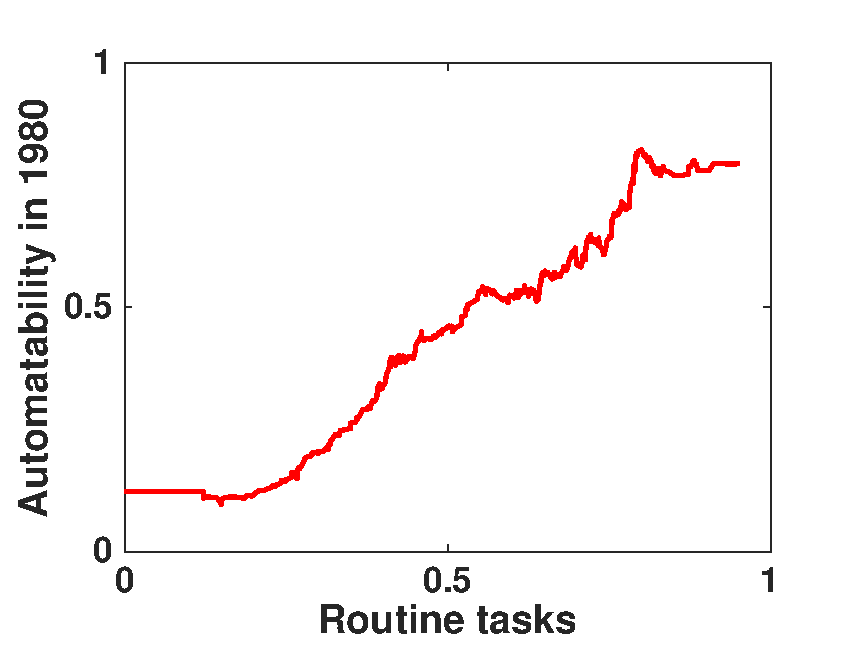
\includegraphics[scale = 0.5]{routine.eps}
\end{subfigure}%
%\hspace*{0.05\textwidth}
\begin{subfigure}{0.48\textwidth}
\centering
	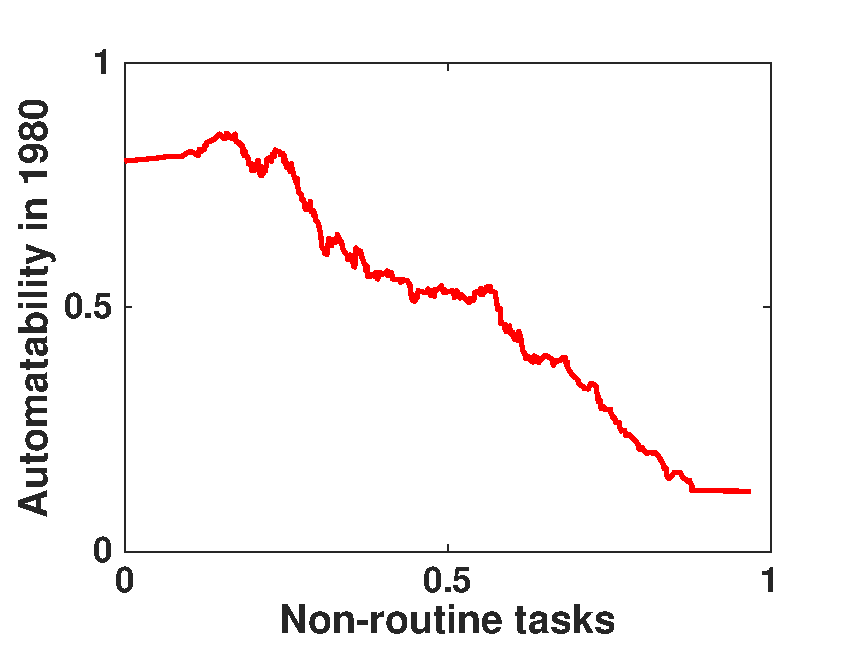
\includegraphics[scale = 0.5]{non-routine.eps}
\end{subfigure}

\caption{Averaged probability of computerisation vs. \\categorical task measurements in 1980.}
\label{fig:1980cat}
\end{figure}

Figure \ref{fig:1980cat} are the probability for routine tasks and non-routine tasks in general. Again, the categorical task scores are the sum of all variables in each category. The plot is generated by applying a moving average filter over all occupations. There is a steady increase in probability with higher routine tasks and reverse trend in non-routine tasks. The plots matches the conclusion of David Autor et al.\cite{david2001skill} that computers substitutes workers in routine jobs while complements those in non-routine jobs. 


To further prove that the result is correct, the employment data from IPUMS\cite{IPUMS1990} is compared with the probability of computerisation in 1980. If the predictions are  correct, occupations with high probability of computerisation should have decreased in employment rate\footnotemark. If we exclude the extreme values ( with more than 0.25 percent change in employment rate) and fit it with a least square line, we could see a clear trend giving negative relationship between probability and employment change in Figure\ref{fig:labor_change}.


\footnotetext{Employment rate here refers to the percentage of population that is working in a job.}

 
\begin{figure}[htb]
\centering
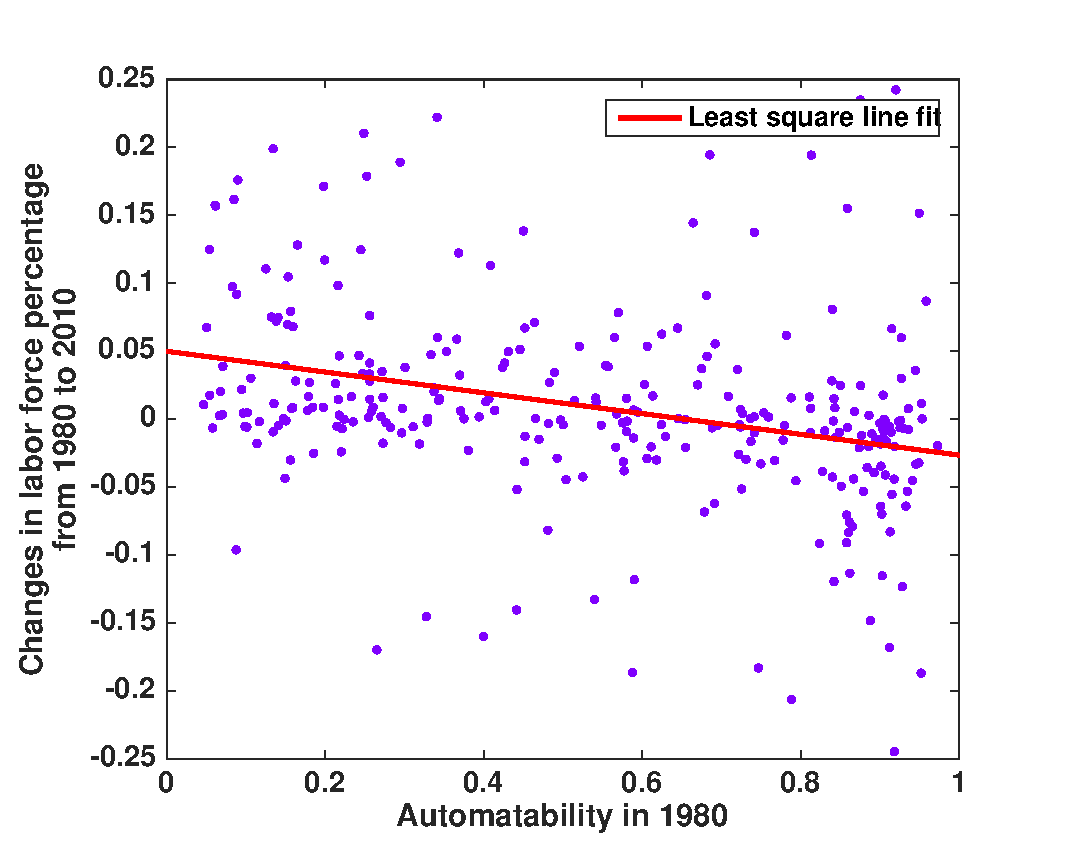
\includegraphics[scale=0.7]{labor_change.eps}
\caption{Change in employment rate from 1980 to 2010 vs probability of computerisation in 1980. Each point represents an occupation }
\label{fig:labor_change}
\end{figure}

If we divide the result into low, medium, and high probability range, the average changes in employment rate for each automatability level can be computed in Table \ref{tab:labor_change}. As expected, high probability of computerisation results in decrease in employment. 

\begin{table}
\centering
\begin{tabular}{c c}
\thickhline
Probability of computerisation & Change in employment rate \\ \hline
low                        & $0.037\pm 0.005 $                  \\
medium                     & $0.002\pm 0.003$                      \\
high                       & $-0.011\pm 0.006$                      \\ \thickhline
\end{tabular}
\centering
\caption{Mean and standard deviation of changes in employment rate \\based on each level of automatability}
\label{tab:labor_change}
\end{table} 

On the other hand, the fact that the employment rate of low automatability jobs are more likely to have increased fits well to the opinion of Brynjolfsson and McAfee\cite{brynjolfsson2012race}. They argued that computerisation will not make people useless. Instead, it will shift the labor market so that more people are working on those tasks that computers are not good at. As long as human learns to use computers to help them with other non-computerisable tasks, that is to keep computers being complementary instead of being a substitute, they will not be a threat to human jobs. This means two things. First, as computers become cheaper and smarter, more people will use computers as their complementary tool for their jobs today. Second, new jobs will be created by using more powerful computers as infrastructure. The only case we need to worry is when the rate of computer development become faster than the rate at which human creating and adapting to new jobs. If that happens, the employment rate of human race would be expected to decrease.


\section{Changes in probability from 1980 to 2010}
To study how probability of computerisation has changed from 1980 to 2010, the change in probability for each occupation is collected. The histogram is shown in Figure \ref{fig:hist}. 

\begin{figure}[!htb]
\centering
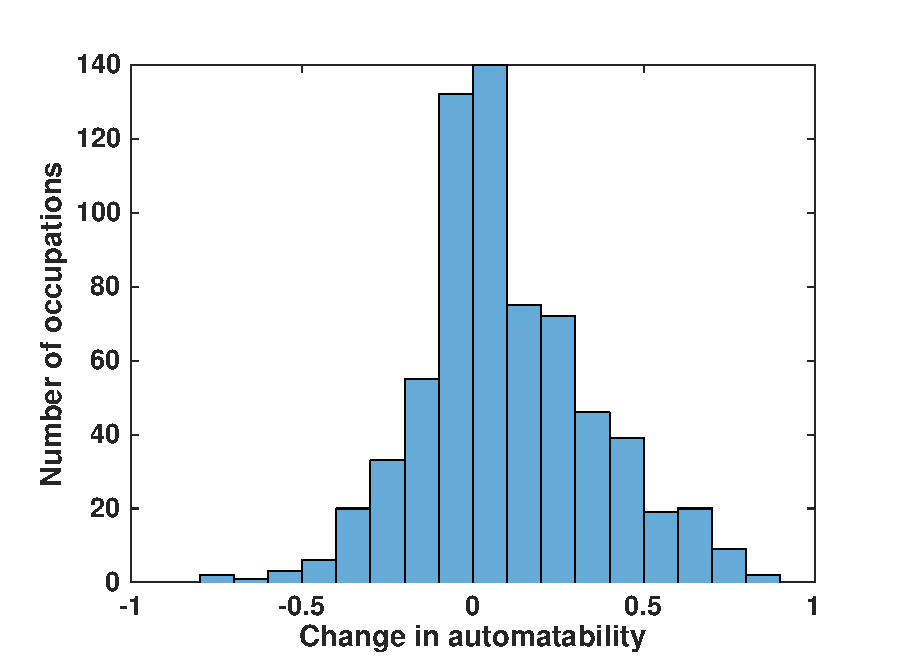
\includegraphics[scale=0.75]{hist.eps}
\caption{Change in probability from 1980 to 2010 histogram. }
\label{fig:hist}
\end{figure}

There are more occupations with increased probability than with decreased probability. It can be explained in two possible ways. First, the same labels are applied to two different data sets. If routine task components in occupations, especially the highly automatable ones, has decreased through the 30 years, an occupation with label '1' in 2010 may have lower score in routine tasks than that occupation in 1980. This results in a lower requirement in routine task score for an occupation in 2010 to be classified as 'automatable'. Second, two data sets are using different measuring systems. The 2010 data set takes account of 9 features while the 1980 data have 26 variables. The 1980 data set have measured more features and therefore it may give very different results. 


\chapter{Conclusion}
\rhead{}
In this project, the probabilities of future computerisation for occupations in 2010 and 1980 are computed using Gaussian process classification. The result is analysed in two major steps. First, the results are used to find the relation between automatability and the tasks required for each occupation. Second, the results of 1980 occupations are used to predict the employment change which is then examined on the actual history data. In conclusion, jobs with relatively high score in routine tasks, compared to score of non-routine tasks, are more susceptible to computerisation. In contrast, jobs with relatively high demand in non-routine tasks are less likely to be automated. 

However, this is just a short term prediction based on current technology. Resistance in automation for non-routine tasks will no longer exist when its related technical bottlenecks are broken.  This has already happened in some non-routine tasks. Self-driving cars are emerging these days with the development of artificial intelligence. Robots are learning to write novels. Being affected by these new technologies, the negative relation between non-routine tasks and automatability is no longer hold for non-routine manual tasks. There is no reason for us to not believe that similar things would happen in other areas. 

Although the development of technology will make machine more capable of human works, it does not need to become a disaster. The book \textit{The new division of labor: How computers are creating the next job market}\cite{levy2012new} believes that what technology do is to shift the the tasks that human workers perform. The investment in computers resulted in striking decrease in routine task frequency while complex communications and expert thinking frequencies increased more than expected. The development of technology is not a threat to human workers as a whole. Although it does decline the labor force of occupations that involves routine tasks that computers can perform, at the same time, it pushed more people to take more complex tasks that computers cannot do. 



\section{Limitations}
There are potential errors in the employment prediction. First, the crosswalk files did not make perfect matches for occupation from 1980 and 2010 because of change of occupational structures. Some 2010 occupations can not find correspondences in 1980 simply because they did not exist at that time. Some may find multiple correspondences because jobs branch and merge over time. Therefore it may be better if more precise labels could be determined individually other than relying on crosswalks to transfer from the 2010 labels. In addition, the mismatch of occupations causes a small amount of data loss when comparing probabilities, which may or may not have affected the final results.  

Other factors such as politics may also affect the actual automatability. This project only discusses the computerisation from a technical point of view -- which occupations are at a risk to be automated given current technology. Also, it is not taking into account the possible future developments in new technology. The breaking of engineering bottlenecks in the future, obviously, will again change the image of computerisation probability. 



\rhead{}
 




\begin{flushleft}
\bibliographystyle{apalike}
\bibliography{4YP}
\end{flushleft}



\newpage
\appendix

\chapter{Probabilities of computerisation}  \label{App:results_all} 
\renewcommand{\headrulewidth}{0pt}
\singlespacing
\renewcommand{\arraystretch}{1.0}
\begingroup
\fontsize{10pt}{12pt}\selectfont

\centering

\begin{longtable}{ p{.45\textwidth} p{.030\textwidth} p{.030\textwidth}  p{.1\textwidth}  p{.1\textwidth}  p{.13\textwidth} } 

\thickhline\\
\multicolumn{2}{c }{Occupation} & & \multicolumn{2}{  c }{\parbox{.20\textwidth}{Probability of computerisation}} & \multirow{2}{*}{\parbox{.13\textwidth}{Change in employment rate}}\\
\cmidrule{1-2} \cmidrule{4-5}\\
  Name & label & & 2010 & 1980 &\\
  \cmidrule{1-2} \cmidrule{4-6}\\
 \endfirsthead
 

 \thickhline\\
\multicolumn{2}{c }{Occupation} & & \multicolumn{2}{ c }{\parbox{.20\textwidth}{Probability of computerisation}} & \multirow{2}{*}{\parbox{.13\textwidth}{Change in employment rate}}\\
\cmidrule{1-2} \cmidrule{4-5}\\
 Name & Label & & 2010 & 1980 &\\
  \cmidrule{1-2} \cmidrule{4-6}\\
 \endhead
 

Recreational Therapists	&		&	&	0.036	&	0.256	&	0.04100	\\
Emergency Management Directors	&		&	&	0.041	&	0.141	&	0.07500	\\
Psychologists All Other	&		&	&	0.042	&	0.106	&	0.03000	\\
First-Line Supervisors of Mechanics Installers and Repairers	&		&	&	0.046	&	0.301	&	0.03800	\\
Social and Community Service Managers	&	0	&	&	0.047	&	0.129	&		\\
Healthcare Social Workers	&		&	&	0.048	&	0.051	&	0.06700	\\
Mental Health Counselors	&		&	&	0.048	&	0.198	&	0.17100	\\
Occupational Therapists	&		&	&	0.049	&	0.256	&	0.02800	\\
Audiologists	&		&	&	0.051	&	0.256	&	0.03300	\\
Physicians and Surgeons	&	0	&	&	0.051	&		&		\\
Instructional Coordinators	&		&	&	0.052	&	0.103	&	0.70800	\\
Dentists General	&	0	&	&	0.053	&	0.070	&	0.00300	\\
First-Line Supervisors of Fire Fighting and Prevention Workers	&		&	&	0.053	&	0.216	&	0.01400	\\
Elementary School Teachers Except Special Education	&		&	&	0.054	&	0.075	&	0.29500	\\
Speech-Language Pathologists	&		&	&	0.054	&	0.256	&	0.03300	\\
Clergy	&	0	&	&	0.066	&	0.157	&	0.07900	\\
Educational Guidance School and Vocational Counselors	&		&	&	0.067	&	0.198	&	0.17100	\\
Career/Technical Education Teachers Secondary School	&		&	&	0.068	&	0.088	&	-0.09600	\\
Preschool Teachers Except Special Education	&	0	&	&	0.071	&	0.054	&	0.12500	\\
Secondary School Teachers Except Special and Career/Technical Education	&		&	&	0.071	&	0.088	&	-0.09600	\\
Sales Managers	&		&	&	0.081	&	0.068	&	0.02000	\\
Public Relations and Fundraising Managers	&		&	&	0.084	&	0.068	&	0.02000	\\
Logisticians	&		&	&	0.085	&	0.426	&	0.04100	\\
Pharmacists	&		&	&	0.086	&	0.163	&	0.02800	\\
Registered Nurses	&	0	&	&	0.086	&		&		\\
First-Line Supervisors of Production and Operating Workers	&		&	&	0.097	&	0.196	&	-0.60900	\\
Rehabilitation Counselors	&		&	&	0.098	&	0.198	&	0.17100	\\
Chief Executives	&	0	&	&	0.098	&	0.158	&	0.40700	\\
Materials Engineers	&		&	&	0.099	&	0.254	&	0.00100	\\
Education Administrators Preschool and Childcare Center/Program	&	0	&	&	0.099	&	0.085	&	0.16200	\\
Materials Scientists	&		&	&	0.099	&	0.319	&	-0.01800	\\
Fashion Designers	&	0	&	&	0.100	&	0.165	&	0.12800	\\
First-Line Supervisors of Office and Administrative Support Workers	&		&	&	0.100	&	0.450	&	0.13800	\\
Civil Engineers	&	0	&	&	0.102	&	0.233	&	0.01600	\\
Photographers	&		&	&	0.102	&	0.135	&	0.01100	\\
Marriage and Family Therapists	&	0	&	&	0.115	&	0.198	&	0.17100	\\
Interior Designers	&		&	&	0.116	&	0.165	&	0.12800	\\
Writers and Authors	&		&	&	0.120	&	0.342	&	0.06000	\\
Meeting Convention and Event Planners	&	0	&	&	0.123	&	0.129	&		\\
Chiropractors	&		&	&	0.133	&	0.179	&	0.01700	\\
Multimedia Artists and Animators	&		&	&	0.133	&	0.157	&	0.00800	\\
Lawyers	&	0	&	&	0.139	&	0.090	&	0.17600	\\
Landscape Architects	&	0	&	&	0.142	&	0.054	&	0.01800	\\
Social Scientists and Related Workers All Other	&		&	&	0.149	&	0.406	&	0.01500	\\
First-Line Supervisors of Correctional Officers	&		&	&	0.150	&	0.245	&	0.12500	\\
Commercial and Industrial Designers	&		&	&	0.152	&	0.165	&	0.12800	\\
Broadcast News Analysts	&		&	&	0.162	&	0.184	&	0.00900	\\
Occupational Therapy Assistants	&		&	&	0.163	&	0.256	&	0.02800	\\
Substance Abuse and Behavioral Disorder Counselors	&	0	&	&	0.174	&	0.198	&	0.17100	\\
Fine Artists Including Painters Sculptors and Illustrators	&		&	&	0.182	&	0.157	&	0.00800	\\
Graphic Designers	&		&	&	0.185	&	0.165	&	0.12800	\\
Chefs and Head Cooks	&	0	&	&	0.196	&	0.252	&	0.17900	\\
First-Line Supervisors of Non-Retail Sales Workers	&		&	&	0.201	&	0.112	&	0.76200	\\
Radio and Television Announcers	&	0	&	&	0.206	&	0.235	&	-0.00200	\\
Electrical Engineers	&		&	&	0.210	&	0.149	&	-0.04400	\\
Compliance Officers	&	0	&	&	0.214	&	0.515	&	0.01400	\\
Dancers	&		&	&	0.246	&	0.329	&	0.00100	\\
Childcare Workers	&	0	&	&	0.247	&	0.400	&		\\
Licensed Practical and Licensed Vocational Nurses	&		&	&	0.249	&	0.095	&	0.02200	\\
Healthcare Practitioners and Technical Workers All Other	&	0	&	&	0.251	&		&		\\
Petroleum Engineers	&		&	&	0.252	&	0.394	&	0.00200	\\
Animal Trainers	&		&	&	0.253	&	0.788	&	-0.20600	\\
Physicists	&	0	&	&	0.266	&	0.215	&	-0.00500	\\
Hairdressers Hairstylists and Cosmetologists	&	0	&	&	0.266	&	0.138	&	0.07200	\\
Computer Hardware Engineers	&		&	&	0.292	&	0.149	&	-0.04400	\\
Agents and Business Managers of Artists Performers and Athletes	&		&	&	0.292	&	0.097	&	0.00400	\\
Career/Technical Education Teachers Middle School	&		&	&	0.327	&	0.075	&	0.29500	\\
First-Line Supervisors of Retail Sales Workers	&		&	&	0.329	&	0.112	&	0.76200	\\
Geographers	&		&	&	0.333	&	0.406	&	0.01500	\\
Financial Analysts	&		&	&	0.340	&	0.295	&	0.18900	\\
Concierges	&	0	&	&	0.352	&	0.580	&	0.01500	\\
Athletes and Sports Competitors	&	0	&	&	0.371	&	0.088	&	0.09200	\\
Zoologists and Wildlife Biologists	&	0	&	&	0.377	&	0.159	&	0.00800	\\
Firefighters	&		&	&	0.390	&	0.216	&	0.01400	\\
Financial Specialists All Other	&		&	&	0.397	&	0.295	&	0.18900	\\
Private Detectives and Investigators	&		&	&	0.415	&	0.199	&	0.11700	\\
Architectural and Civil Drafters	&		&	&	0.453	&	0.858	&	-0.09100	\\
Economists	&	0	&	&	0.456	&	0.446	&	0.05100	\\
Judges Magistrate Judges and Magistrates	&	0	&	&	0.459	&	0.054	&		\\
Surveyors	&	1	&	&	0.461	&	0.217	&		\\
Computer Programmers	&		&	&	0.477	&	0.645	&	0.32900	\\
Advertising Sales Agents	&		&	&	0.483	&	0.180	&	0.02700	\\
Ambulance Drivers and Attendants Except Emergency Medical Technicians	&		&	&	0.483	&	0.782	&	0.06200	\\
Judicial Law Clerks	&	1	&	&	0.484	&	0.685	&	0.19400	\\
Merchandise Displayers and Window Trimmers	&		&	&	0.508	&	0.165	&	0.12800	\\
Plumbers Pipefitters and Steamfitters	&	0	&	&	0.510	&	0.504	&	-0.04500	\\
Costume Attendants	&		&	&	0.517	&	0.565	&	0.06000	\\
Agricultural Engineers	&		&	&	0.522	&	0.243	&	0.04700	\\
Aerospace Engineering and Operations Technicians	&		&	&	0.539	&	0.681	&	0.09100	\\
Radiation Therapists	&		&	&	0.540	&	0.256	&	0.04100	\\
Machinists	&		&	&	0.559	&	0.590	&	-0.11800	\\
Life Physical and Social Science Technicians All Other	&		&	&	0.560	&	0.681	&	0.09100	\\
Transportation Storage and Distribution Managers	&	0	&	&	0.560	&	0.726	&	0.00400	\\
Market Research Analysts and Marketing Specialists	&	1	&	&	0.568	&	0.141	&	0.07500	\\
Cost Estimators	&	1	&	&	0.574	&	0.129	&		\\
First-Line Supervisors of Farming Fishing and Forestry Workers	&		&	&	0.578	&	0.812	&	-0.01000	\\
Social Science Research Assistants	&		&	&	0.580	&	0.681	&	0.09100	\\
Personal Financial Advisors	&		&	&	0.596	&	0.295	&	0.18900	\\
Commercial Pilots	&		&	&	0.605	&	0.403	&	0.01300	\\
Flight Attendants	&	0	&	&	0.612	&	0.370	&	0.03200	\\
Fire Inspectors and Investigators	&		&	&	0.615	&	0.216	&	0.01400	\\
Police Fire and Ambulance Dispatchers	&		&	&	0.627	&	0.521	&	0.05400	\\
Mine Shuttle Car Operators	&		&	&	0.627	&	0.903	&	-0.11500	\\
Massage Therapists	&		&	&	0.628	&	0.408	&	0.11300	\\
Purchasing Agents Except Wholesale Retail and Farm Products	&		&	&	0.646	&	0.218	&	0.04700	\\
Correctional Officers and Jailers	&		&	&	0.658	&	0.245	&	0.12500	\\
Court Municipal and License Clerks	&		&	&	0.661	&	0.843	&	0.00800	\\
Dental Assistants	&		&	&	0.668	&	0.198	&	0.00900	\\
Avionics Technicians	&		&	&	0.670	&	0.500	&	-0.00400	\\
Civil Engineering Technicians	&	1	&	&	0.678	&	0.681	&	0.09100	\\
Bartenders	&		&	&	0.681	&	0.750	&	-0.03300	\\
Crossing Guards	&		&	&	0.692	&	0.594	&	0.00500	\\
Electronic Equipment Installers and Repairers Motor Vehicles	&		&	&	0.693	&	0.500	&	-0.00400	\\
Recreational Vehicle Service Technicians	&		&	&	0.698	&	0.541	&	0.01600	\\
Motorboat Operators	&	1	&	&	0.700	&	0.589	&	-0.01400	\\
Electrical and Electronics Drafters	&	1	&	&	0.707	&	0.858	&	-0.09100	\\
Computer Automated Teller and Office Machine Repairers	&		&	&	0.727	&	0.464	&	0.07100	\\
Barbers	&		&	&	0.728	&	0.273	&	-0.01800	\\
Hunters and Trappers	&	0	&	&	0.740	&		&		\\
Dental Hygienists	&		&	&	0.753	&	0.247	&	0.03300	\\
Motorcycle Mechanics	&		&	&	0.755	&	0.741	&	0.00200	\\
Cutters and Trimmers Hand	&		&	&	0.758	&	0.913	&	-0.08300	\\
Welding Soldering and Brazing Machine Setters Operators and Tenders	&		&	&	0.761	&	0.888	&	-0.14800	\\
Carpenters	&		&	&	0.761	&	0.328	&	-0.14600	\\
Technical Writers	&	1	&	&	0.778	&	0.218	&	0.00300	\\
Computer-Controlled Machine Tool Operators Metal and Plastic	&	1	&	&	0.782	&	0.603	&	0.02500	\\
Foundry Mold and Coremakers	&		&	&	0.789	&	0.901	&	-0.06400	\\
Motorboat Mechanics and Service Technicians	&		&	&	0.791	&	0.741	&	0.00200	\\
Bus Drivers Transit and Intercity	&	1	&	&	0.803	&	0.682	&	0.04600	\\
Postal Service Mail Carriers	&		&	&	0.807	&	0.953	&	0.00000	\\
Power Plant Operators	&		&	&	0.810	&	0.371	&	0.00600	\\
Sheet Metal Workers	&	1	&	&	0.815	&	0.557	&	0.03900	\\
Light Truck or Delivery Services Drivers	&	1	&	&	0.821	&	0.861	&	-0.07600	\\
Maids and Housekeeping Cleaners	&	0	&	&	0.822	&	0.368	&	0.12200	\\
Laundry and Dry-Cleaning Workers	&		&	&	0.828	&	0.901	&	-0.03500	\\
Personal Care Aides	&		&	&	0.829	&	0.111	&	0.44400	\\
Insurance Sales Agents	&		&	&	0.843	&	0.858	&	-0.07100	\\
Dishwashers	&	1	&	&	0.848	&	0.850	&	0.02500	\\
Accountants and Auditors	&	1	&	&	0.848	&	0.686	&	0.32600	\\
Chemical Plant and System Operators	&		&	&	0.853	&	0.849	&	-0.01000	\\
Human Resources Assistants Except Payroll and Timekeeping	&	1	&	&	0.862	&	0.907	&	-0.01600	\\
Tax Examiners and Collectors and Revenue Agents	&	1	&	&	0.866	&	0.686	&	0.32600	\\
Patternmakers Metal and Plastic	&		&	&	0.868	&	0.778	&	-0.01500	\\
Parking Lot Attendants	&	1	&	&	0.869	&	0.724	&	0.00700	\\
Railroad Brake Signal and Switch Operators	&		&	&	0.869	&	0.827	&	-0.03900	\\
Cooks Fast Food	&	1	&	&	0.870	&	0.252	&	0.17900	\\
Meter Readers Utilities	&	1	&	&	0.872	&	0.859	&	-0.00600	\\
Taxi Drivers and Chauffeurs	&	1	&	&	0.872	&	0.782	&	0.06200	\\
Compensation and Benefits Managers	&		&	&	0.878	&	0.152	&	0.07000	\\
Maintenance Workers Machinery	&		&	&	0.878	&	0.877	&	-0.01200	\\
Forest and Conservation Workers	&		&	&	0.880	&	0.812	&	-0.01000	\\
Nonfarm Animal Caretakers	&		&	&	0.882	&	0.720	&	0.03600	\\
Paralegals and Legal Assistants	&	1	&	&	0.886	&	0.685	&	0.19400	\\
Parking Enforcement Workers	&		&	&	0.890	&	0.245	&	0.12500	\\
Bus Drivers School or Special Client	&		&	&	0.901	&	0.682	&	0.04600	\\
Medical Transcriptionists	&	1	&	&	0.907	&	0.664	&	0.14400	\\
Sewing Machine Operators	&	1	&	&	0.907	&	0.708	&	-0.45400	\\
Real Estate Brokers	&		&	&	0.913	&	0.337	&	0.02000	\\
Credit Analysts	&	1	&	&	0.914	&	0.295	&	0.18900	\\
Butchers and Meat Cutters	&		&	&	0.915	&	0.725	&	-0.05100	\\
Helpers--Carpenters	&		&	&	0.915	&	0.875	&	0.02500	\\
Food and Tobacco Roasting Baking and Drying Machine Operators and Tenders	&		&	&	0.915	&	0.375	&	0.00000	\\
Electrical and Electronic Equipment Assemblers	&	1	&	&	0.916	&	0.927	&	-0.52900	\\
Bicycle Repairers	&		&	&	0.917	&	0.541	&	0.01600	\\
Gaming Dealers	&	1	&	&	0.919	&	0.565	&	0.06000	\\
Couriers and Messengers	&	1	&	&	0.921	&	0.915	&	0.06700	\\
File Clerks	&	1	&	&	0.923	&	0.911	&	-0.00500	\\
Cement Masons and Concrete Finishers	&		&	&	0.927	&	0.741	&	-0.01000	\\
Refuse and Recyclable Material Collectors	&		&	&	0.928	&	0.924	&	-0.00200	\\
Claims Adjusters Examiners and Investigators	&	1	&	&	0.929	&	0.741	&	0.13700	\\
Industrial Truck and Tractor Operators	&	1	&	&	0.930	&	0.861	&	-0.07600	\\
Waiters and Waitresses	&	0	&	&	0.934	&	0.587	&	-0.18700	\\
Mail Clerks and Mail Machine Operators Except Postal Service	&		&	&	0.935	&	0.934	&	-0.05300	\\
Payroll and Timekeeping Clerks	&		&	&	0.935	&	0.973	&	-0.02000	\\
Radio Operators	&		&	&	0.938	&	0.688	&	-0.00600	\\
Farm Labor Contractors	&	1	&	&	0.939	&	0.812	&	-0.01000	\\
Woodworking Machine Setters Operators and Tenders Except Sawing	&		&	&	0.939	&	0.935	&	0.00800	\\
Legal Secretaries	&		&	&	0.942	&	0.294	&	-0.56700	\\
Postal Service Clerks	&		&	&	0.943	&	0.860	&	-0.08400	\\
Switchboard Operators Including Answering Service	&	1	&	&	0.945	&	0.912	&	-0.16800	\\
Shoe Machine Operators and Tenders	&		&	&	0.945	&	0.866	&	-0.04400	\\
Driver/Sales Workers	&		&	&	0.946	&	0.861	&	-0.07600	\\
Telephone Operators	&		&	&	0.946	&	0.912	&	-0.16800	\\
Data Entry Keyers	&	1	&	&	0.948	&	0.945	&	-0.03300	\\
Shipping Receiving and Traffic Clerks	&		&	&	0.951	&	0.862	&	-0.11300	\\
Insurance Underwriters	&	1	&	&	0.951	&	0.839	&	0.02800	\\
Pesticide Handlers Sprayers and Applicators Vegetation	&		&	&	0.952	&	0.626	&	0.27600	\\
Cashiers	&	1	&	&	0.954	&	0.776	&	0.31900	\\
Credit Authorizers Checkers and Clerks	&	1	&	&	0.956	&	0.692	&	0.05500	\\
Loan Officers	&	1	&	&	0.957	&	0.295	&	0.18900	\\
Library Technicians	&		&	&	0.961	&	0.482	&	-0.00300	\\
Tax Preparers	&		&	&	0.962	&	0.295	&	0.18900	\\
Telemarketers	&		&	&	0.962	&	0.663	&	-1.65100	\\
\hline 

\caption{Probability of computerisation in 1980 and 2010 \\(some 1980 reaults are missing for being not able to find correspondences using crosswalk files).} 
\label{tab:myfirstlongtable}


\end{longtable}
\endgroup


\end{spacing}
\end{document}